% -*- Mode:TeX -*-

%% IMPORTANT: The official thesis specifications are available at:
%%            http://libraries.mit.edu/archives/thesis-specs/
%%
%%            Please verify your thesis' formatting and copyright
%%            assignment before submission.  If you notice any
%%            discrepancies between these templates and the 
%%            MIT Libraries' specs, please let us know
%%            by e-mailing thesis@mit.edu

%% The documentclass options along with the pagestyle can be used to generate
%% a technical report, a draft copy, or a regular thesis.  You may need to
%% re-specify the pagestyle after you \include  cover.tex.  For more
%% information, see the first few lines of mitthesis.cls. 

%\documentclass[12pt,vi,twoside]{mitthesis}
%%
%%  If you want your thesis copyright to you instead of MIT, use the
%%  ``vi'' option, as above.
%%
%\documentclass[12pt,twoside,leftblank]{mitthesis}
%%
%% If you want blank pages before new chapters to be labelled ``This
%% Page Intentionally Left Blank'', use the ``leftblank'' option, as
%% above. 

\documentclass[12pt,twoside]{mitthesis}
\usepackage{lgrind}

%% Packages not included in the template
%% next three for using inkscape pdf+latex output
\usepackage{import}
\usepackage{color}
\usepackage{graphicx}
\graphicspath{{figures/}}
%% for chemistry formatting
\usepackage{mhchem}

%% These have been added at the request of the MIT Libraries, because
%% some PDF conversions mess up the ligatures.  -LB, 1/22/2014
\usepackage{cmap}
\usepackage[T1]{fontenc}
\pagestyle{plain}

%% This bit allows you to either specify only the files which you wish to
%% process, or `all' to process all files which you \include.
%% Krishna Sethuraman (1990).

%%\typein [\files]{Enter file names to process, (chap1,chap2 ...), or `all' to
%%process all files:}
%%\def\all{all}
%%\ifx\files\all \typeout{Including all files.} \else \typeout{Including only \files.} \includeonly{\files} \fi

\begin{document}

% -*-latex-*-
% 
% For questions, comments, concerns or complaints:
% thesis@mit.edu
% 
%
% $Log: cover.tex,v $
% Revision 1.8  2008/05/13 15:02:15  jdreed
% Degree month is June, not May.  Added note about prevdegrees.
% Arthur Smith's title updated
%
% Revision 1.7  2001/02/08 18:53:16  boojum
% changed some \newpages to \cleardoublepages
%
% Revision 1.6  1999/10/21 14:49:31  boojum
% changed comment referring to documentstyle
%
% Revision 1.5  1999/10/21 14:39:04  boojum
% *** empty log message ***
%
% Revision 1.4  1997/04/18  17:54:10  othomas
% added page numbers on abstract and cover, and made 1 abstract
% page the default rather than 2.  (anne hunter tells me this
% is the new institute standard.)
%
% Revision 1.4  1997/04/18  17:54:10  othomas
% added page numbers on abstract and cover, and made 1 abstract
% page the default rather than 2.  (anne hunter tells me this
% is the new institute standard.)
%
% Revision 1.3  93/05/17  17:06:29  starflt
% Added acknowledgements section (suggested by tompalka)
% 
% Revision 1.2  92/04/22  13:13:13  epeisach
% Fixes for 1991 course 6 requirements
% Phrase "and to grant others the right to do so" has been added to 
% permission clause
% Second copy of abstract is not counted as separate pages so numbering works
% out
% 
% Revision 1.1  92/04/22  13:08:20  epeisach

% NOTE:
% These templates make an effort to conform to the MIT Thesis specifications,
% however the specifications can change.  We recommend that you verify the
% layout of your title page with your thesis advisor and/or the MIT 
% Libraries before printing your final copy.
\title{A 64 Channel 3T Array Coil for Highly Accelerated Fetal Imaging at 22 Weeks of Pregnancy}

\author{Mark H. Spatz}
% If you wish to list your previous degrees on the cover page, use the 
% previous degrees command:
%       \prevdegrees{A.A., Harvard University (1985)}
% You can use the \\ command to list multiple previous degrees
%       \prevdegrees{B.S., University of California (1978) \\
%                    S.M., Massachusetts Institute of Technology (1981)}
\department{Department of Electrical Engineering and Computer Science}

% If the thesis is for two degrees simultaneously, list them both
% separated by \and like this:
% \degree{Doctor of Philosophy \and Master of Science}
\degree{Master of Engineering in Electrical Engineering and Computer Science}

% As of the 2007-08 academic year, valid degree months are September, 
% February, or June.  The default is June.
\degreemonth{February}
\degreeyear{2017}
\thesisdate{Feb 3, 2017}

%% By default, the thesis will be copyrighted to MIT.  If you need to copyright
%% the thesis to yourself, just specify the `vi' documentclass option.  If for
%% some reason you want to exactly specify the copyright notice text, you can
%% use the \copyrightnoticetext command.  
%\copyrightnoticetext{\copyright IBM, 1990.  Do not open till Xmas.}

% If there is more than one supervisor, use the \supervisor command
% once for each.
\supervisor{Lawrence L. Wald}{Professor of Radiology, Harvard Medical School}

% This is the department committee chairman, not the thesis committee
% chairman.  You should replace this with your Department's Committee
% Chairman.
\chairman{Christopher Terman}{Chairman, Masters of Engineering Thesis Committee}

% Make the titlepage based on the above information.  If you need
% something special and can't use the standard form, you can specify
% the exact text of the titlepage yourself.  Put it in a titlepage
% environment and leave blank lines where you want vertical space.
% The spaces will be adjusted to fill the entire page.  The dotted
% lines for the signatures are made with the \signature command.
\maketitle

% The abstractpage environment sets up everything on the page except
% the text itself.  The title and other header material are put at the
% top of the page, and the supervisors are listed at the bottom.  A
% new page is begun both before and after.  Of course, an abstract may
% be more than one page itself.  If you need more control over the
% format of the page, you can use the abstract environment, which puts
% the word "Abstract" at the beginning and single spaces its text.

%% You can either \input (*not* \include) your abstract file, or you can put
%% the text of the abstract directly between the \begin{abstractpage} and
%% \end{abstractpage} commands.

% First copy: start a new page, and save the page number.
\cleardoublepage
% Uncomment the next line if you do NOT want a page number on your
% abstract and acknowledgments pages.
% \pagestyle{empty}
\setcounter{savepage}{\thepage}
\begin{abstractpage}
% $Log: abstract.tex,v $
% Revision 1.1  93/05/14  14:56:25  starflt
% Initial revision
% 
% Revision 1.1  90/05/04  10:41:01  lwvanels
% Initial revision
% 
%
%% The text of your abstract and nothing else (other than comments) goes here.
%% It will be single-spaced and the rest of the text that is supposed to go on
%% the abstract page will be generated by the abstractpage environment.  This
%% file should be \input (not \include 'd) from cover.tex.
In this thesis, I designed and implemented a compiler which performs
optimizations that reduce the number of low-level floating point operations
necessary for a specific task; this involves the optimization of chains of
floating point operations as well as the implementation of a ``fixed'' point
data type that allows some floating point operations to simulated with integer
arithmetic.  The source language of the compiler is a subset of C, and the
destination language is assembly language for a micro-floating point CPU.  An
instruction-level simulator of the CPU was written to allow testing of the
code.  A series of test pieces of codes was compiled, both with and without
optimization, to determine how effective these optimizations were.

\end{abstractpage}

% Additional copy: start a new page, and reset the page number.  This way,
% the second copy of the abstract is not counted as separate pages.
% Uncomment the next 6 lines if you need two copies of the abstract
% page.
% \setcounter{page}{\thesavepage}
% \begin{abstractpage}
% % $Log: abstract.tex,v $
% Revision 1.1  93/05/14  14:56:25  starflt
% Initial revision
% 
% Revision 1.1  90/05/04  10:41:01  lwvanels
% Initial revision
% 
%
%% The text of your abstract and nothing else (other than comments) goes here.
%% It will be single-spaced and the rest of the text that is supposed to go on
%% the abstract page will be generated by the abstractpage environment.  This
%% file should be \input (not \include 'd) from cover.tex.
In this thesis, I designed and implemented a compiler which performs
optimizations that reduce the number of low-level floating point operations
necessary for a specific task; this involves the optimization of chains of
floating point operations as well as the implementation of a ``fixed'' point
data type that allows some floating point operations to simulated with integer
arithmetic.  The source language of the compiler is a subset of C, and the
destination language is assembly language for a micro-floating point CPU.  An
instruction-level simulator of the CPU was written to allow testing of the
code.  A series of test pieces of codes was compiled, both with and without
optimization, to determine how effective these optimizations were.

% \end{abstractpage}

\cleardoublepage

\section*{Acknowledgments}

This is the acknowledgements section.  You should replace this with your
own acknowledgements.

%%%%%%%%%%%%%%%%%%%%%%%%%%%%%%%%%%%%%%%%%%%%%%%%%%%%%%%%%%%%%%%%%%%%%%
% -*-latex-*-

% Some departments (e.g. 5) require an additional signature page.  See
% signature.tex for more information and uncomment the following line if
% applicable.
% % -*- Mode:TeX -*-
%
% Some departments (e.g. Chemistry) require an additional cover page
% with signatures of the thesis committee.  Please check with your
% thesis advisor or other appropriate person to determine if such a 
% page is required for your thesis.  
%
% If you choose not to use the "titlepage" environment, a \newpage
% commands, and several \vspace{\fill} commands may be necessary to
% achieve the required spacing.  The \signature command is defined in
% the "mitthesis" class
%
% The following sample appears courtesy of Ben Kaduk <kaduk@mit.edu> and
% was used in his June 2012 doctoral thesis in Chemistry. 

\begin{titlepage}
\begin{large}
This doctoral thesis has been examined by a Committee of the Department
of Chemistry as follows:

\signature{Professor Jianshu Cao}{Chairman, Thesis Committee \\
   Professor of Chemistry}

\signature{Professor Troy Van Voorhis}{Thesis Supervisor \\
   Associate Professor of Chemistry}

\signature{Professor Robert W. Field}{Member, Thesis Committee \\
   Haslam and Dewey Professor of Chemistry}
\end{large}
\end{titlepage}


\pagestyle{plain}
  % -*- Mode:TeX -*-
%% This file simply contains the commands that actually generate the table of
%% contents and lists of figures and tables.  You can omit any or all of
%% these files by simply taking out the appropriate command.  For more
%% information on these files, see appendix C.3.3 of the LaTeX manual. 
\tableofcontents
\newpage
\listoffigures
\newpage
\listoftables


\chapter{Introduction}
MRI is increasingly used in addition to ultrasound to evaluate potential fetal disorders in routine clinical practice.
Indeed, MRI provides a higher soft tissue contrast than ultrasound in the fetus and reproductive organs. MRI also has
the potential to provide valuable physiological information through spectroscopic and diffusion weighted imaging. In
practice, the problem of unpredictable and nonrigid fetal motion limits fetal MRI to fast single shot T2 weighted
sequences such as HASTE, which have poor tissue contrast, low SNR, and cannot provide detailed physiological information.

High density arrays are needed to minimize acquisition times and maximize SNR. A standard fetal MRI protocol employs a
spine array and a flexible body array to reach a total of approximately 34 channels. This limits the acceleration
factors that can be achieved. Additionally, these general purpose coils are often unable to completely conform to the
varied anatomy of pregnant patients, leaving some receive elements distant to the abdomen. In this work, we designed,
built, and tested a semi-adjustable anatomically shaped 64 channel array coil for fetal imaging at 22 weeks of pregnancy
on a 3T MAGNETOM Skyra system (Siemens Healthcare GmbH, Erlangen, Germany) .

\newcommand{\uvec}[1]{\bm{\hat{#1}}}
\newcommand{\bvec}[1]{\bm{\vec{#1}}}

\chapter{Background}
Magnetic resonance imaging is, as the name suggests, enabled by the phenomenon of magnetic resonance.

\section{Origin of MR signal}

\subsection{Nuclear Spins}
Spin is a quantum mechanical property that describes a particle's intrinsic angular momentum. Atoms with an odd
number of protons or neutrons possess net nuclear spin, and therefore have mutually aligned angular momentum $\bvec{S}$
and magnetic dipole moment $\bvec{\mu}= \gamma \bvec{S}$, where $\gamma$ is the gyromagnetic ratio: a known constant
defined for every nucleus. Hydrogen (\ce{^{1}_{1}H}) is such an atom, having one proton and no neutrons. Along a given
axis, hydrogen spins are quantized to $\pm \frac{\hbar}2$.  Therefore, hydrogen dipole moments are likewise quantized to
$\pm \gamma \frac{\hbar}{2}$ (eq. \ref{eq:dipole}).

\begin{equation}\label{eq:dipole}
    \mu = \pm \gamma \frac{\hbar}{2}
\end{equation}

\subsection{Spins in the Presence of External Magnetic Fields}
In the presence of a strong polarizing field $\bvec{B_0}$ pointing in the $z$ direction and with magnitude $B_0$, the
potential energy of a spin with dipole moment $\bvec{\mu}$ is the dot product between the two vectors.

\begin{equation}\label{eq:spin_energy}
    E = - \bvec{\mu} \cdot \bvec{B_0}
\end{equation}

Because $\mu$ is quantized, there is a gap $\Delta E$ between realizable energy states.

\begin{equation}\label{eq:delta_E}
    \Delta E = \gamma \hbar B_0
\end{equation}

\subsubsection{Polarization}
Spins tend to settle in the low energy state, pointing in the direction of $\bvec{B_0}$. However, at room temperature,
thermal energy vastly exceeds the energy gap between the two states, and the ratio of spins aligned with $\bvec{B_0}$
($n_+$) to those anti aligned ($n_-$) is described by the Boltzmann distribution in eq. \ref{eq:boltzmann}. For hydrogen
($\gamma = \frac{42.58}{2\pi} \frac{MHz}{T}$) at room temperature ($T=273 K$) at a field strength of $3T$, $\Delta E =
5.283 \times 10^{-7} eV$, and $\frac{n_-}{n_+} \approx (1 - 2.25 \times 10^{-5})$. This relatively tiny fraction of
excess spin polarization is the source of the NMR signal. Luckily, there are $3.3428 \times 10^{23}$ protons in a gram
of water, resulting in $7.5 \times 10^{18}$ aligned spins per gram under the previously stated conditions. Since living
things tend to contain mostly water, the proposal of MRI is still promising.

\begin{equation}\label{eq:boltzmann}
    \frac{n_-}{n_+} = \exp(-\frac{\Delta E}{k T}) = \exp(-\frac{\gamma \hbar B_0}{k T})
\end{equation}

In a large population of spins, the net magnetic dipole moment per unit volume is termed $\bvec{M}$. In equilibrium, it
is the product of the volumetric spin density $N$, the magnitude of a single spin dipole moment $\mu$, and the excess
fraction of aligned spins. It points in the same direction as $\bvec{B_0}$ and has magnitude $M_0$. Using the first two
terms of a taylor series expansion of the Boltzmann distribution, we can approximate $M_0$ as eq. \ref{eq:M}.

\begin{equation}\label{eq:M}
    M_0 = N \cdot \mu \cdot (1-\exp(-\frac{\Delta E}{k T})) \approx \frac{N \gamma^2 \hbar^2 B_0}{2 k T}
\end{equation}

\subsection{Spin Dynamics}
In equilibrium, $\bvec{M}$ comes to point in the direction $\bvec{B_0}$ with magnitude $M_0$. But the next step will be
to tip $\bvec{M}$ off of the $z$ axis so that it has a component in the $x$-$y$ plane. The observed behavior will then
be time varying.

\subsubsection{Precession}
A single magnetic dipole $\bvec{\mu}$ with mutually aligned angular momentum $\bvec{S}$ placed in an external magnetic
field $\bvec{B}$ will experience a torque $\bvec{\mu} \times \bvec{B}$. Multiplying this torque by $\gamma$ gives an
expression for the time rate of change of $\bvec{\mu}$, eq. \ref{eq:dipole_precession}. Eq. \ref{eq:dipole_precession}
shows $\bvec{\mu}$ moving in a direction perpendicular to both itself and $\bvec{B}$, i.e. precessing about $\bvec{B}$.
The frequency of this precession is $\omega_L$ in eq. \ref{eq:precession_freq}.

\begin{equation}\label{eq:dipole_precession}
    \frac{d \bvec{\mu}}{dt} = \bvec{\mu} \times \gamma \bvec{B}
\end{equation}

\begin{equation}\label{eq:precession_freq}
    \omega_L = \gamma \cdot B
\end{equation}

A population of dipole moments precessing in synchrony gives a net magnetization $\bvec{M}$ that also precesses at
$\omega_L$.

\subsubsection{Longitudinal Relaxation}
Define the component of $\bvec{M}$ that is parallel to $\bvec{B_0}$ as $\bvec{M_z}$. In equilibrium $|\bvec{M_z}| =
M_0$, but immediately following the tipping of $\bvec{M}$ into the $x$-$y$ plane by an angle $\alpha$ at time $t=0$,
$\bvec{M_z}$ is reduced to a value shown in eq. \ref{eq:mz_postflip}.

\begin{equation}\label{eq:mz_postflip}
    \bvec{M_z}(t=0+) = \cos(\alpha) \cdot \bvec{M_z}(0-)
\end{equation}

$\bvec{M_z}$ then begins to exponentially recover to its equilibrium magnitude of $M_0$. The time constant associated
with this longitudinal recovery is termed $T_1$. $T_1$ is dependent on the tissue or material being imaged, but also has
a positive dependence on $B_0$ field strength.

\begin{equation}\label{eq:t1_decay}
    \bvec{M_{z}}(t) = \uvec{k} M_0 + (\bvec{M_{z}}(0+) - \uvec{k} M_0) \cdot \exp(-\frac{t}{T_1})
\end{equation}

\subsubsection{Transverse Relaxation}
Define the component of $\bvec{M}$ that is perpendicular to $\bvec{B_0}$ as $\bvec{M_{xy}}$. In equilibrium,
$\bvec{M_{xy}} = 0$.  Immediately following the tipping of $\bvec{M}$ onto the $x$ axis by an angle $\alpha$ at
time $t=0$, $\bvec{M_{xy}}$ is as shown in eq. \ref{eq:mxy_postflip}. Individual spins begin to dephase as soon as they
are tipped into the $x$-$y$ plane, and so the net transverse magnetization $\bvec{M_{xy}}$ experiences exponential
decay, as shown in eq. \ref{eq:t2_decay}. The time constant associated with this transverse decay is termed $T_2$, and
is a property of the tissue or material being imaged.

\begin{equation}\label{eq:mxy_postflip}
    \bvec{M_{xy}}(t=0+) = \uvec{i}\sin(\alpha) \cdot |\bvec{M_z}(0-)|
\end{equation}

\begin{equation}\label{eq:t2_decay}
    \bvec{M_{xy}}(t) = \bvec{M_{xy}}(0+) \cdot \exp(-\frac{t}{T_2})
\end{equation}

\subsection{Bloch Equation}
Assembled together, the spin dynamics described above form the Bloch equation, shown in eq. \ref{eq:bloch}. The complete
Bloch equation describes the behavior of spins in a generalized external magnetic field $\bvec{B}$ that is the sum of
the main field $B_0$, the RF field $B_1$, and the spatially varying gradient fields $G$. 

\begin{equation}\label{eq:bloch}
    \frac{d \bvec{M}}{dt} = \bvec{M} \times \gamma \bvec{B} - \frac{M_x \uvec{i} + M_y \uvec{j}}{T_2} - \frac{(M_z - M_0)
    \uvec{k}}{T_1}
\end{equation}

\section{Signal Equation}
The NMR signal arises from the precessing transverse component of the magnetization vector. As we begin to focus solely
on $\bvec{M_{xy}}$, I will follow the convention used by Nishimura \cite{nishimura} and define a new variable $M$ that
represents the transverse magnetization as a function of location and time with single complex number.

\begin{equation}\label{eq:M_complex}
    M(\bvec{r},t) \equiv |\bvec{M_x}| + j |\bvec{M_y}|
\end{equation}

\subsection{Signal Detection Through Faraday Induction}
The wire loop antenna is the most commonly used receive element in clinical MRI. It works by directly coupling to the
field produced by the transverse magnetization of the sample under test. The precessing magnetization produces a time
varying magnetic flux piercing the surface defined by the loop, which induces a voltage $\epsilon$ around the loop
through Faraday induction.

\begin{equation}\label{eq:faraday_induction}
    \epsilon = - \frac{d \Phi_B}{dt} = -\frac{d}{dt} \iint_A B(\bvec{r},t) dA
\end{equation}

A loop antenna has spatially varying sensitivity to spins. If a unit current through the loop produces a field
$\bvec{B_1}$ at location $\bvec{r}$ in the sample, then magnetization $\bvec{M}$ at that location produces a flux of
$\bvec{B_1} \cdot \bvec{M}$ through the loop.  \cite{Hoult1979}. Citing linearity, we can find an expression for the
total voltage induced around the loop by summing the individual contributions from every location in the sample volume.

\begin{equation}\label{eq:reciprocity}
    \epsilon = -\frac{d}{dt} \iiint_V \bvec{B_1}(\bvec{r}) \cdot \bvec{M}(\bvec{r}) d\bvec{r}
\end{equation}

The voltage around the loop depends on the time derivative of a volume integral over the entire sample volume. At this
point, it is clear why only the precessing transverse magnetization is of interest for signal detection. Substituting
our complex variable $M$ into eq. \ref{eq:reciprocity}, and replacing $\bvec{B_1}$ with a more general complex sensitivity
function $C(\bvec{r})$ that also accounts for spatially dependent signal phase, we get the beginnings of the signal
equation

\begin{equation}\label{eq:signal_1}
    \epsilon = -\frac{d}{dt} \iiint_V C(\bvec{r}) \cdot M(\bvec{r},t) d\bvec{r}
\end{equation}

\section{Fourier Encoding}

\subsection{Gradient Fields}
Spatial encoding in traditional MRI is achieved by applying spatially varying gradient fields on top of the main field,
as shown in eq. \ref{eq:gradients}. Just like $\bvec{B_0}$, $\bvec{G}$ points in the $\uvec{k}$ direction. Unlike
$\bvec{B_0}$, $\bvec{G}$ varies as a function of space and time.

\begin{equation}\label{eq:gradients}
    \bvec{B} = (B_0 + G(\bvec{r},t))\uvec{k}
\end{equation}

After an initial flip resulting in a spatial magnetization distribution $M(\bvec{r},t=0)$, spins begin precess under the
influence of $G$, as described in \ref{eq:phase_enc}. After a time $t$, spins at a location $\bvec{r}$ have accrued
excess phase in proportion to the time integral of $G(\bvec{r},t)$.

\begin{equation}\label{eq:phase_enc}
    M(\bvec{r},t) = M(\bvec{r},t=0) e^{-j \gamma B_0 t} exp(-j \gamma \int_0^t G(\bvec{r},\tau) d \tau)
\end{equation}

Plugging this expression for $M$ into eq. \ref{eq:signal_1}, making the assumption that $B_0 >> G$ so that all spins
precess at a frequency of approximately $\omega_L = \gamma B_0$, and dividing by $e^{-j \omega_L t}$ to downconvert to
baseband, we extend the signal equation to describe the effect of gradient fields.

\begin{equation}\label{signal_2}
    s(t) = - j \omega_L \iiint_V C(\bvec{r}) M(\bvec{r},t=0) exp(-j \gamma \int_0^t G(\bvec{r},\tau)
    d\tau)
\end{equation}

If we constrain ourselves to linear encoding gradients, such that

\begin{equation}\label{linear_gradient}
    G(\bvec{r}=x\uvec{i} + y\uvec{j} + z\uvec{k},t) = G_x(t) x + G_x(t) y + G_z(t) z 
\end{equation}

and then define three $k$ variables to descbibe the history of $G$ along each axis:

\begin{equation}\label{k_space}
    \begin{aligned}
        k_x &= \frac{\gamma}{2\pi} \int_0^t G_x(\tau) d\tau\\
        k_y &= \frac{\gamma}{2\pi} \int_0^t G_y(\tau) d\tau\\
        k_z &= \frac{\gamma}{2\pi} \int_0^t G_z(\tau) d\tau
    \end{aligned}
\end{equation}

we come up with the final form of the signal equation:

\begin{equation}\label{eq:signal_3}
    s(t) = - j \omega_L \iiint_V C(\bvec{r}) M(\bvec{r},t=0) e^{-j k_x x} e^{-j k_y y} e^{-j k_z z} dV 
\end{equation}

\subsection{The Fourier Transform}
The Fourier transform breaks down a function into its individual frequency components by taking inner products of that
function with complex exponentials. Its one dimensional form is shown in eq. \ref{eq:fourier_transform}.

\begin{equation}\label{eq:fourier_transform}
    F(k_x) = \int_{-\infty}^{\infty} f(x)e^{-j2\pi k_x x} dx
\end{equation}

Strikingly, eqs. \ref{eq:signal_3} and \ref{eq:fourier_transform} look extremely similar. The effect of our carefully
chosen linear gradient fields has been to set up a physical three dimensional Fourier transform, where we take the inner
product of $M$ with a complex exponential whose phase has a linear dependence on space. Manipulation of $G(t)$ allows us
to visit and sample arbitrary coordinates $(k_x,k_y,k_z)$ in so called "k-space".  By collecting k-space points on a
cartesian grid and obeying certain sampling criteria, we can collect data that directly represents a spatial Fourier
transform of the sample under test, weighted by $C(\bvec{r})$ and $M(\bvec{r},t=0+)$.

\section{Noise in MRI}
\subsection{Thermal Noise}
The signals involved in MRI are very weak, and extreme care is taken to avoid and minimize all possible noise
sources. Thermal noise arising inside the body is, however, unavoidable. When a perfectly conducting wire loop is
brought near an object with finite conductivity, inductive coupling causes a transformed resistance $R_{LOAD}$ to appear
in the loop. $R_{LOAD}$ depends on the geometry and conductivity of the object that is loading the loop, as well as the
strength of the coupling. If $R_{LOAD}$ is measurable, it can be used to quantify the thermal noise voltage that will be be
detected.

\begin{equation}\label{eq:thermal_noise}
    \bar{e_n^2} = 4 k T_{LOAD} R_{LOAD} \Delta f
\end{equation}

If all components of the MR setup are well designed, this innate noise source will dominate over all others.

\subsubsection{Estimating $R_{LOAD}$}

A current $I$ flowing in the loop creates a spatially varying magnetic field $\bvec{B_1}(\bvec{r})$ in the sample below it. If $I$
is sinusoidal, then the changing $\bvec{B_1}$ will create an associated electric field $\bvec{E}$ according to Faraday's
law of induction.

\begin{equation}\label{eq:differential_faraday}
    \nabla \times \bvec{E}(\bvec{r}) = - \frac{\partial \bvec{B_1}(\bvec{r})}{\partial t}
\end{equation}

If we can solve for this $\bvec{E}$, and if we know the conductivity of the sample, we can determine the power
deposition in the sample and model it by $R_{LOAD}$.

\begin{equation}\label{eq:P_sample}
    P_{SAMPLE} = \frac{1}{2} \iiint_V \sigma |\bvec{E}(\bvec{r})|^2 d\bvec{r}
\end{equation} 

\begin{equation}
    R_{LOAD} = \frac{P_{SAMPLE}}{\sqrt{I}} 
\end{equation}

\subsection{Preamp Noise}
Of the noise sources that we can control, the first amplifier in the signal processing chain is most critical. By
faithfully amplifying the weak NMR signal early, the relative impact of noise injected by further transmission and
processing steps is lessened. Here, I follow chapter 10.6 of \cite{lee2004} to derive an optimal source admittance that
optimizes the noise performance of an amplifier.

\subsubsection{Noise Factor}
Noise factor (denoted by $F$) is a parameter that characterizes the noise performance of an amplifier (or mixer, or any other signal
processing block).  It is defined as:

\begin{equation}\label{eq:noise_factor}
    F = \frac{\text{Total Output Noise Power}}{\text{Output Noise Power Due To Source}}
\end{equation}

In systems consisting of multiple blocks (preamplifier, analog filter, mixer, ADC..) it becomes useful to refer to the
logarithm of $F$, so that the noise contribution of cascaded blocks can be represented as a sum. This logarithmic
parameter is called noise figure:

\begin{equation}\label{eq:noise_figure}
    NF = 20 \log_{10}(F)
\end{equation}

\subsubsection{Two Port Noise Model}

A two port model of a noisy amplifier is shown in figure \ref{fig:2port_noise}. The noise behavior of the amplifier is
completely characterized by two input referenced noise sources: a voltage source with mean value $\bar{e}_n$, and a
current source with with mean value $\bar{i}_n$.

\begin{figure}
    \centering
    \input{figures/2port_noise.pdf_tex}
    \caption{Two port model of a noisy preamp connected to a noisy source.}
    \label{fig:2port_noise}
\end{figure}

Connected to the input of the amplifier is a noise current source with input admittance $Y_S$ and mean value
$\bar{i}_s$. The input noise current is assumed to arise purely from the real part of $Y_S$, so the two are related by eq.
\ref{eq:source_admittance}

\begin{equation}\label{eq:source_admittance}
    Re(Y_S) = G_S = \frac{\bar{i_s^2}}{4kT\Delta f}
\end{equation}

We assume that $\bar{i_s}$ statistically independent from $\bar{e_n}$ and $\bar{i_n}$, since they arise inside of
physically distinct devices. Since $\bar{e_n}$ and $\bar{i_n}$ may arise inside of a single transistor, they cannot be
assumed to be uncorrelated.

Using the parameters of this model, we can begin to calculate the amplifier's noise figure. Since we only need to find
the ratio between total noise power and source derived noise power, not the actual values themselves, we can use the
short cut that output power will be proportional to short circuit mean square input current in both cases.

\begin{equation}\label{eq:2port_noisefactor}
    F = \frac{\overline{|i_s + i_n + Y_S e_n|^2}}{\bar{i_s^2}}
\end{equation}

If we expand the squared term in the numerator, we can get rid of cross terms between uncorrelated variables:

\begin{equation}\label{eq:2port_noisefactor_2}
    F = \frac{\bar{i_s^2} + \overline{|i_n + Y_S e_n|^2}}{\bar{i_s^2}}
\end{equation}

The next step is to break up $i_n$ into two parts: $i_{n_u}$ which is uncorrelated with $e_n$, and $i_{n_c}$ which is
completely correlated to $e_n$. The correlation coefficient takes the form of a complex transadmittance $Y_C$, as it is a ratio between
a current and a voltage.

\begin{equation}\label{eq:cor_uncoor}
    i_n = i_{n_u} + i_{n_c} = i_{n_u} + Y_C e_n
\end{equation}

Making this substitution and again removing uncorrelated cross terms, eq. \ref{eq:2port_noisefactor_2} becomes:

\begin{equation}\label{eq:2port_noisefactor_3}
    F = 1 + \frac{\bar{i_u^2} + |Y_S + Y_C|^2 \bar{e_n^2}}{\bar{i_s^2}}
\end{equation}

\subsubsection{Admittance, Conductivity, and Susceptibility}
Before beginning the next section, recall that just as a complex impedance $Z$ can be decomposed into its real
resistance $R$ and imaginary reactance $X$, a complex admittance $Y$ may be decomposed into a conductivity $G$ and
susceptibility $B$:

\begin{equation}\label{eq:admittance}
    \begin{aligned}
        Z &= R + jX\\
        Y &= G + jB
    \end{aligned}
\end{equation}

\subsubsection{Optimal Source Admittance}
There is an optimal value $Y_S$ that will minimize $F$. All that's left to do in finding it is to set up
\ref{eq:2port_noisefactor_3} so that we can take derivatives with respect to $Y_S$ and set them equal to zero.

Replace the admittances $Y_S$ and $Y_C$ with the corresponding conductivities and susceptibilities, then substitute
$\bar{i_s^2} = G_S 4kT\Delta f$ in the denominator. eq. \ref{eq:2port_noisefactor_3} becomes:

\begin{equation}\label{eq:2port_noisefactor_4}
    F = 1 + \frac{\bar{i_u^2} + \big[(G_C+G_S)^2 + (B_C+B_S)^2\big] \bar{e_n^2}}{4kT \Delta f G_s}
\end{equation}

Minimize $F$ with respect to $B_S$:

\begin{equation}\label{eq:partial_B_S}
    \frac{\partial F}{\partial B_S} = \frac{(2 B_C + 2 B_S) \bar{e_n^2}}{4kT\Delta f G_S} \implies B_{S_{OPT}} = -B_C
\end{equation}

Then, minimize $F$ with respect to $G_S$ and plug in $B_{S_{OPT}}$:

\begin{equation}\label{eq:partial_G_S}
    \frac{\partial F}{\partial G_S} = -\frac{\bar{i_u^2} + \bar{e_n^2} \big[{G_C}^2 + (B_C+B_S)^2 \big]}{4kT\Delta f
    {G_S}^2} + \frac{\bar{e_n^2}}{4 kT\Delta f} \implies G_{S_{OPT}} = \sqrt{\frac{\bar{i_u^2}}{\bar{e_n^2}} + G_C^2}
\end{equation}

We have found our optimal source impance $Y_{S_{OPT}}$.

\begin{equation}\label{eq:y_opt}
    Y_{S_{OPT}} =  \sqrt{\frac{\bar{i_u^2}}{\bar{e_n^2}} + G_C^2} - j B_C
\end{equation}

\chapter{Array Design}
\section{Physical Design}
The 22 week fetal array is designed to provide good surface area coverage and close physical fit on a range of body
types at 22 weeks of pregnancy.  It consists of a rigid posterior panel that attaches directly to the patient table and
a group of anterior and lateral panels that can be freely positioned on the patient. The two lateral panels are attached
to the anterior panel with hinges to provide a degree of freedom. The patient facing surfaces of these panels are
modeled after segmented images of a 22 weeks pregnant volunteer. The precise geometry of the hinged panel assembly was
arrived at through iterative fit tests on pregnant volunteers.
 
The coil formers and housings were designed in Rhinoceros (Robert McNeel \& Associates, WA, USA) and printed in
poly carbonate on a Fortus 400mc 3D printer (Stratasys, Ltd., MN, USA).

\begin{figure}
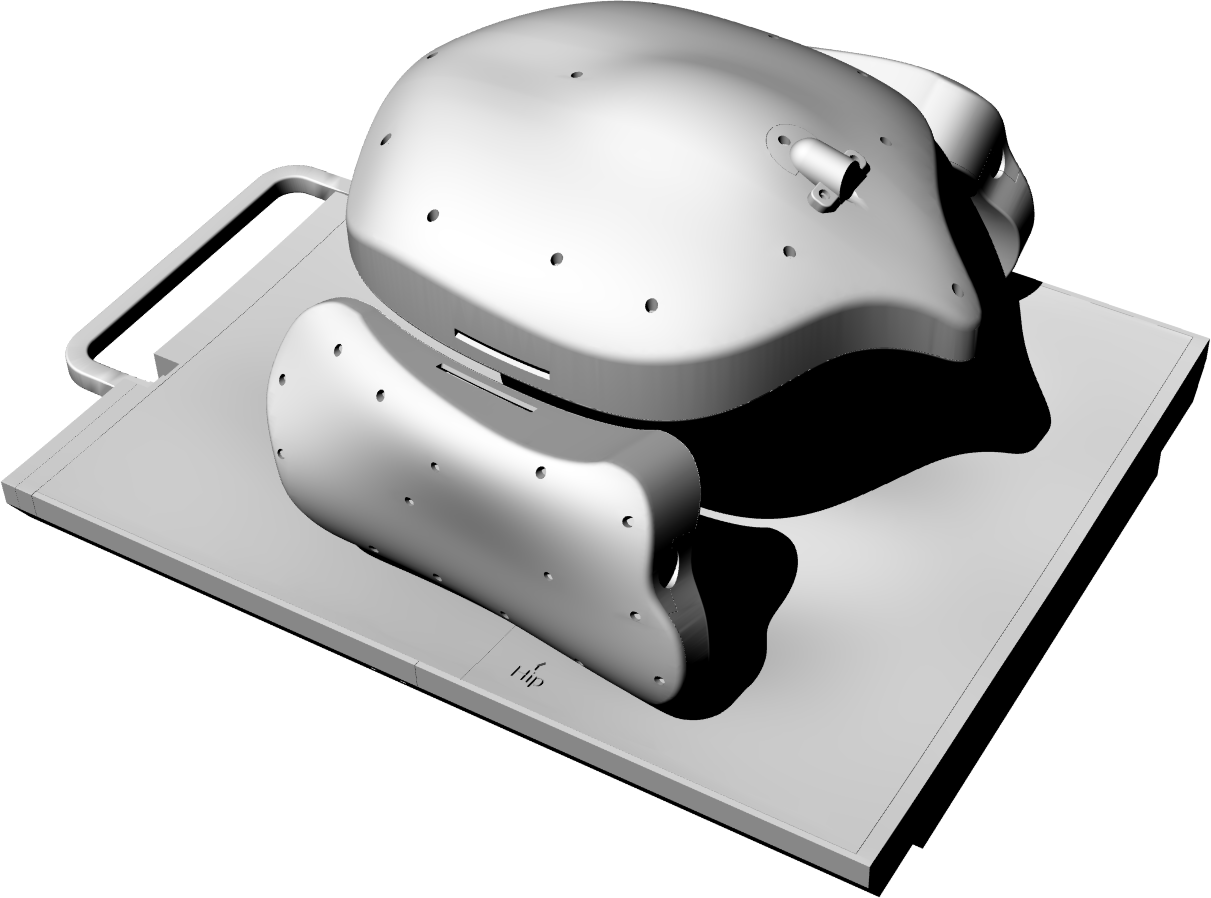
\includegraphics[width=6in]{figures/cad_rendering.png}
\caption{Computer rendering of array panels and housings.}
\label{fig:cad_rendering}
\end{figure}

\section{Array Construction}
The array consists of four distinct groups of coil elements. The posterior panel contains 24 loops, each with a diameter
of approximately 9cm. The anterior panel contains 20 loops, with a median loop diameter of 8cm and with several outliers
in the non-hexagonally tiled area. The two anterior panels contain 10 7cm loops each. The loops in each panel are for
the most part arranged in a hexagonal tiling pattern that allows each loop to be critically overlapped with all of its
neighbors,  thus minimizing inductive coupling between neighboring loops \cite{Roemer94}. The loop layout is shown in
detail in \ref{fig:loop_snr_contributions}.

Individual loops were constructed from 16 gauge tin plated copper wire, with bridges bent into the wires to allow them
to cross each other without touching. A schematic of the loop circuitry is shown in \ref{fig:loop_schematic}. Chapter 4
contains a detailed explanation of the function of the loop circuit.

The finished coil is shown in figure \ref{fig:assembled_view} posed on the pregnant abdomen phantom used extensively
in testing. A view of the internal construction and wiring is shown in figure \ref{fig:internals_composite}.

\begin{figure}
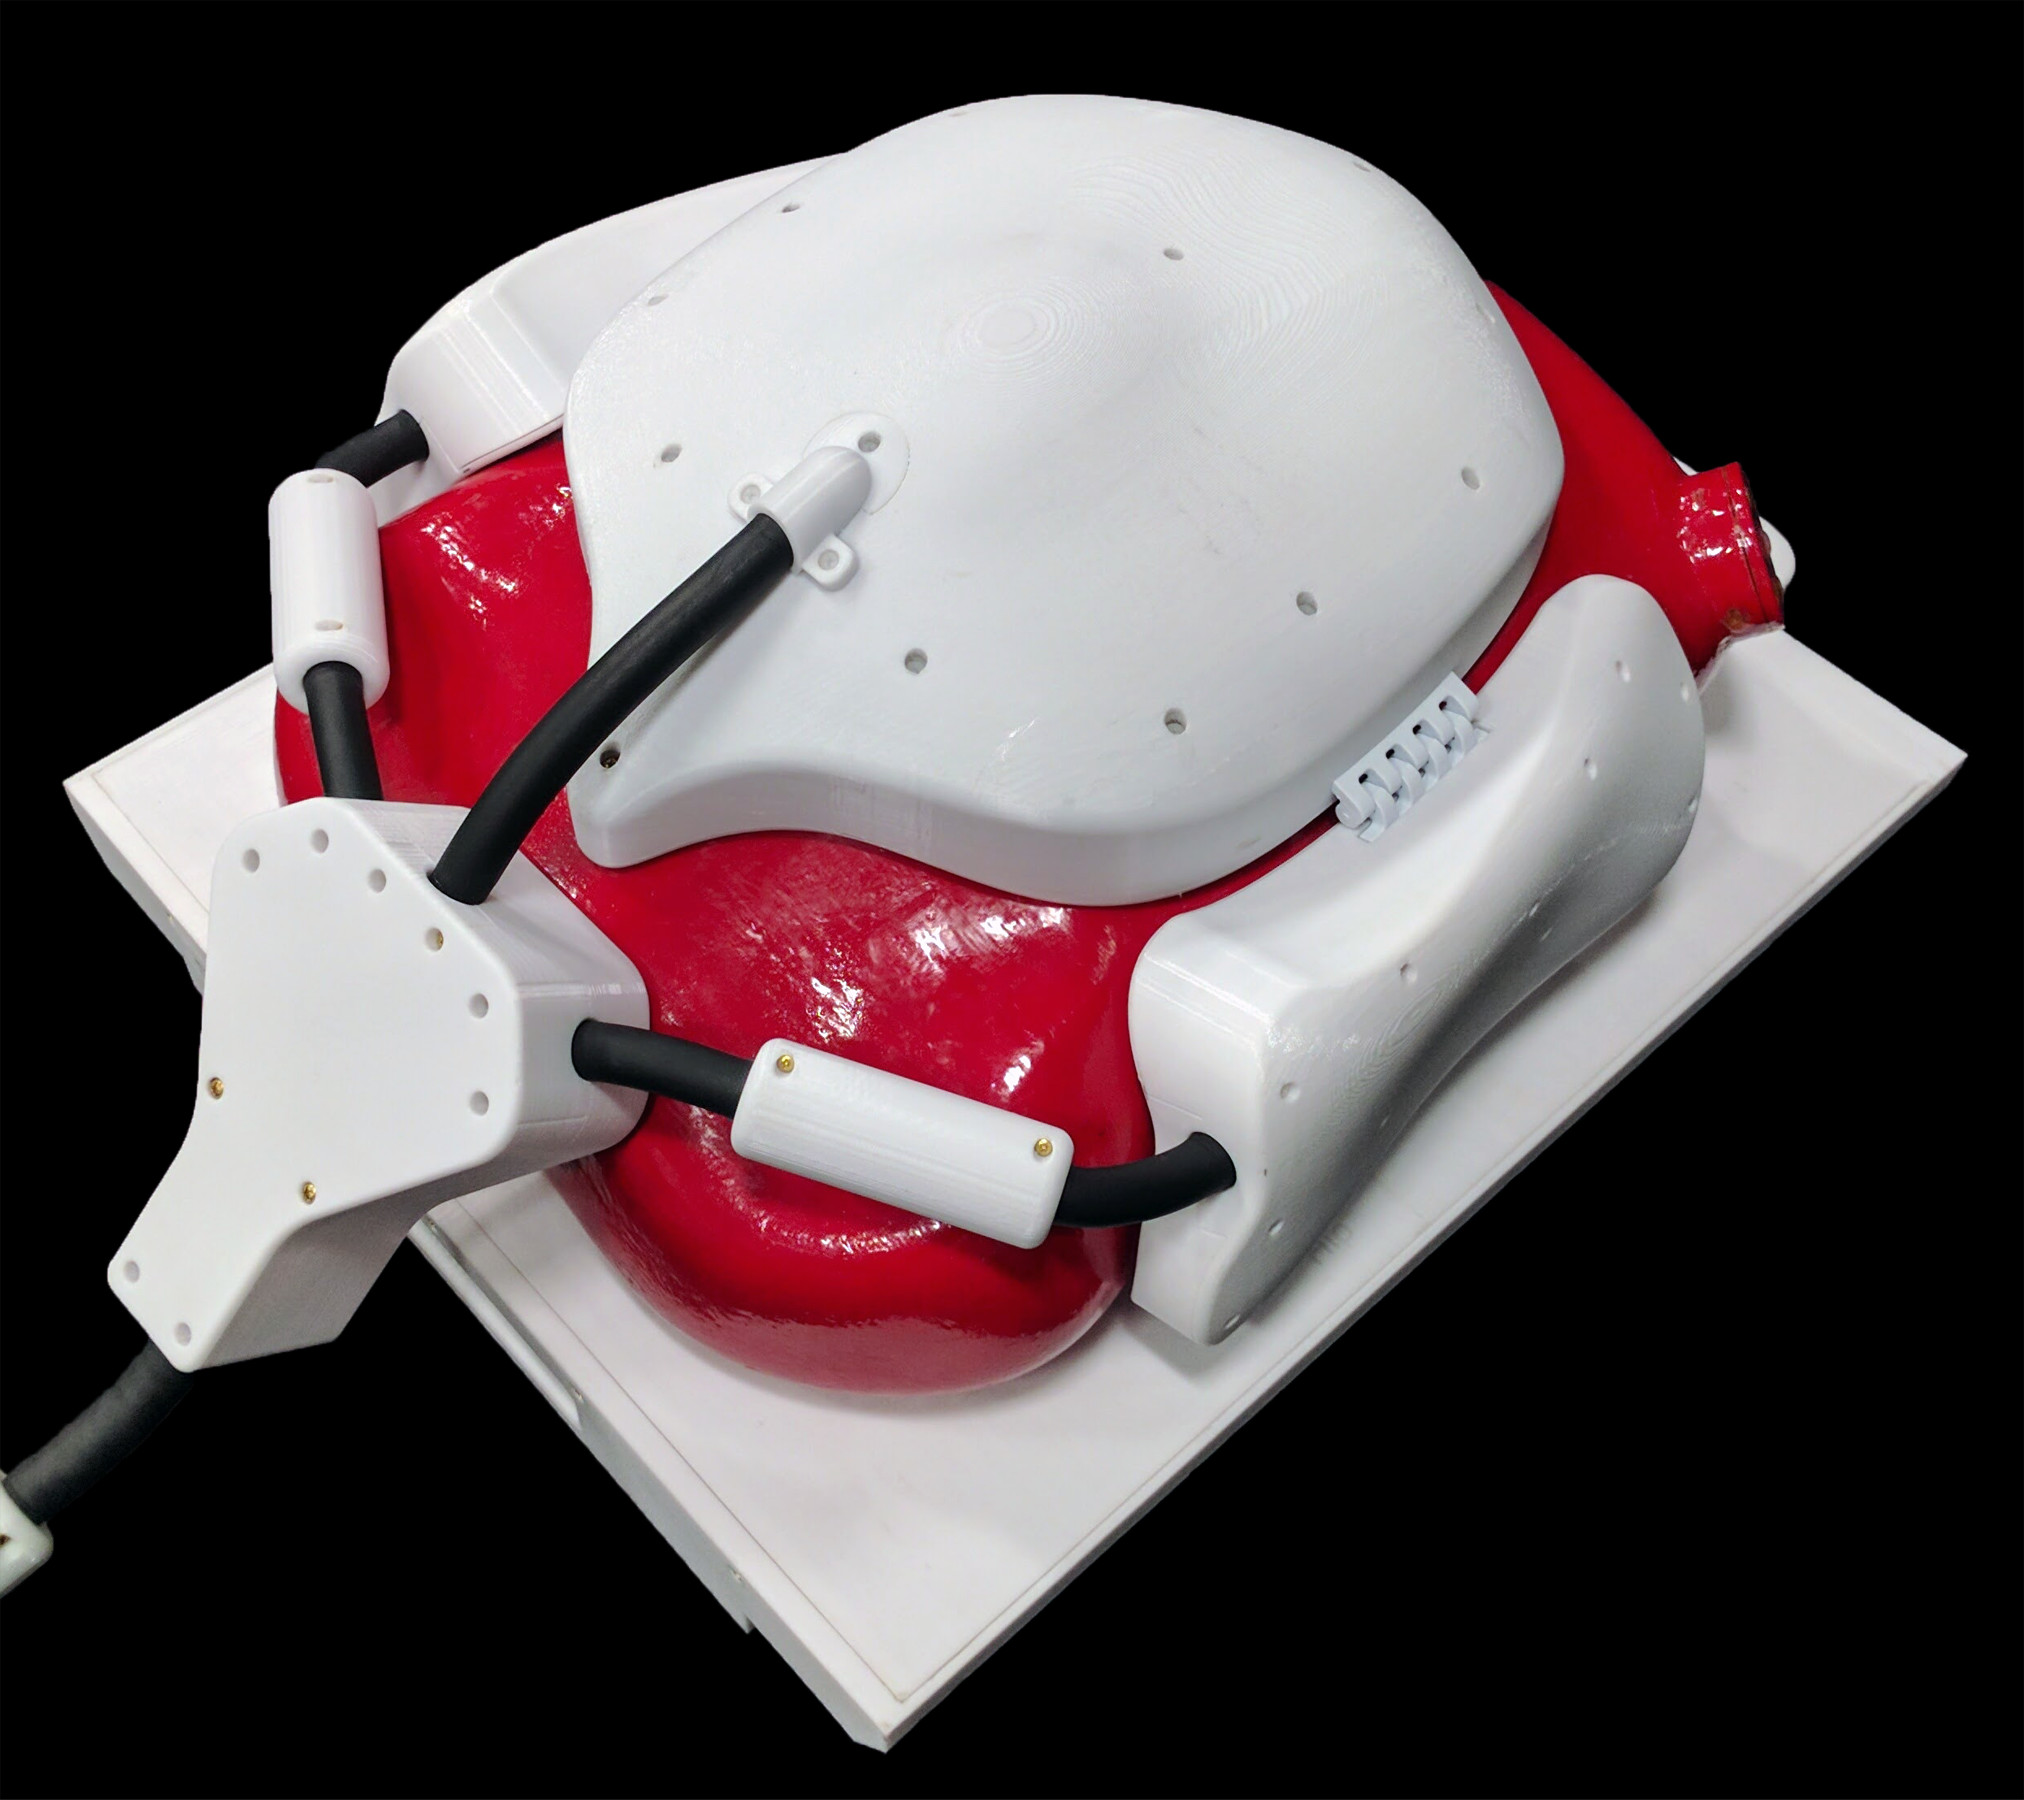
\includegraphics[width=6in]{figures/assembled_view.jpg}
\caption{Finished coil, posed on 22 week pregnant abdomen phantom.}
\label{fig:assembled_view}
\end{figure}

\begin{figure}
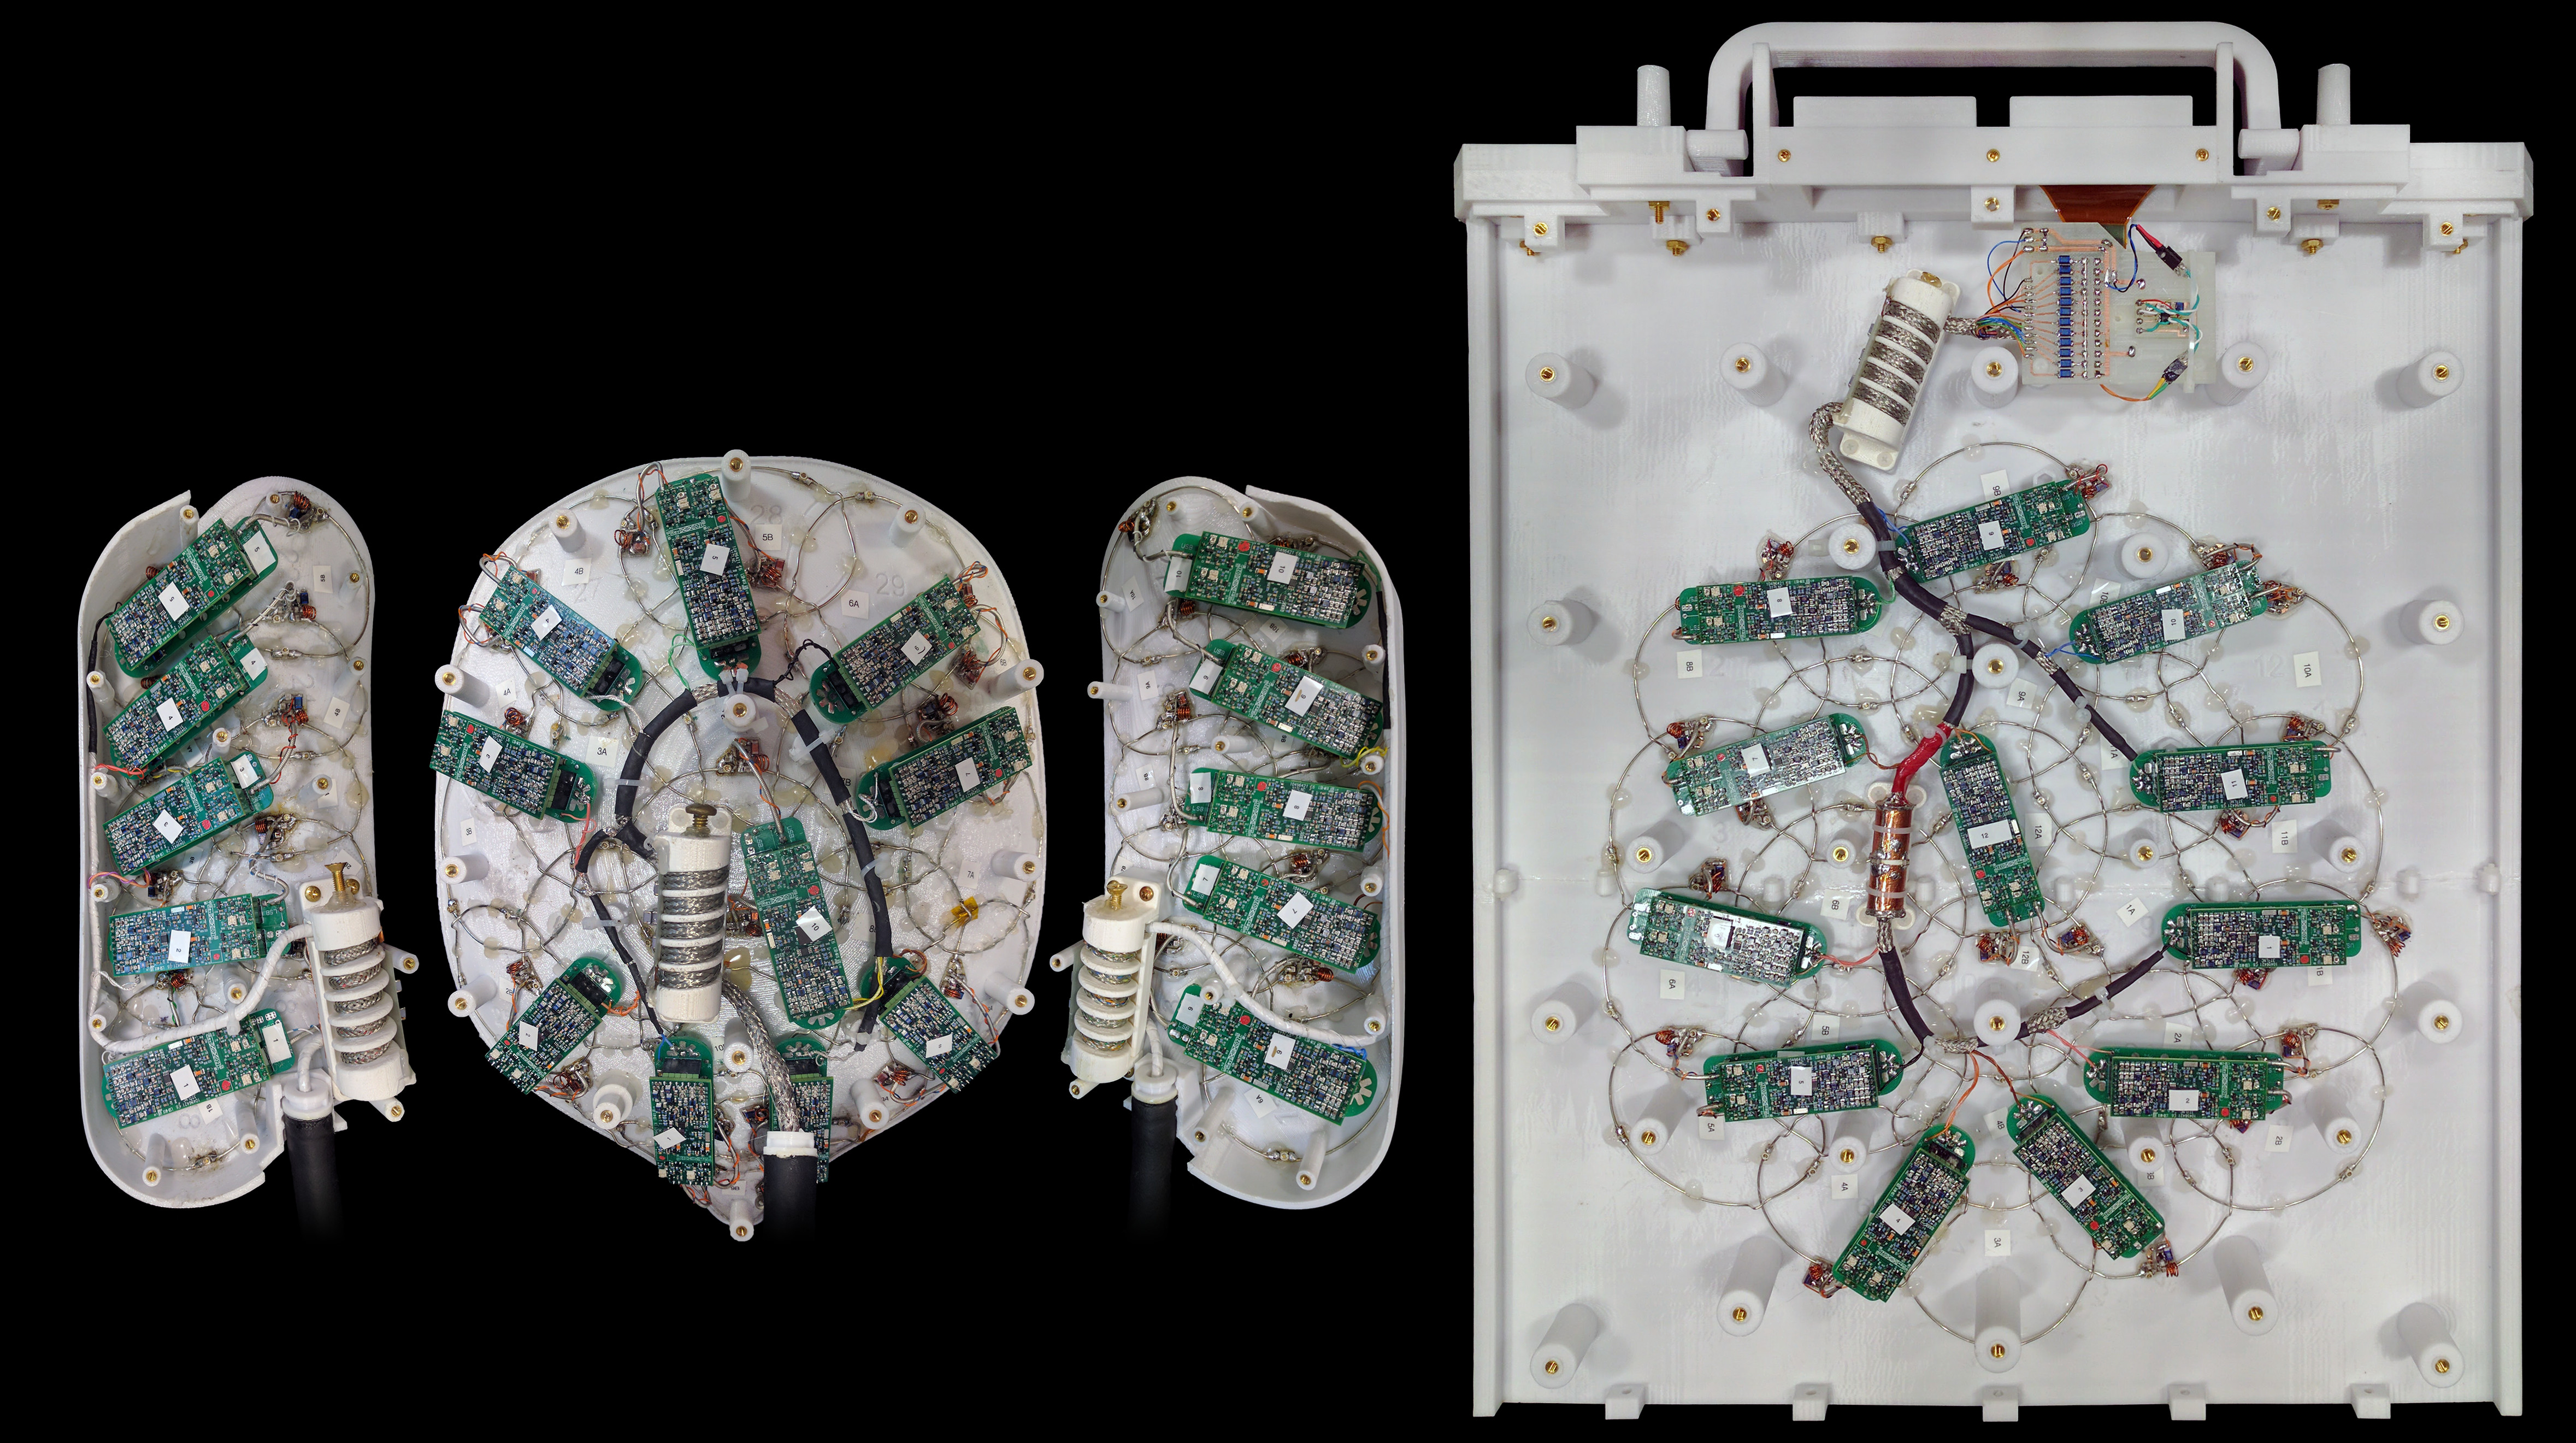
\includegraphics[width=6in]{figures/internals_composite.jpg}
\caption{View of internal array construction and wiring.}
\label{fig:internals_composite}
\end{figure}

\section{Cable Traps}
Precautions must be taken to prevent large currents from developing on internal and external wiring during the RF
transmit phase. Such uncontrolled currents could pose a fire/safety hazard, and at the very least would interfere with
the sequence being run. Common mode chokes spaced every 20cm on all internal and external prevent the induced currents
from growing too large. Due to the high magnetic field the array operates in, ferrite chokes are not an option. Instead,
tuned resonant traps are constructed. Two types of traps were used in this array.

\subsection{Helical Traps}
The operation of the resonant helical traps visible in fig. \ref{fig:internals_composite} is easy to understand.  The
jacketed wire bundle is wound around a helical former, forming an air core inductor. High voltage capacitors are then
connected across the turns of the inductor, forming a parallel LC tank. At resonance, the trap presents a high impedance
to common mode currents flowing in the jacket.  This kind of trap can hold off hundreds of volts, and has a high Q. It
is used as the first cable trap inside each array panel, and inside the table plug.

\subsection{Bazooka Trap}

The bazooka trap can be thought of as a physically short bazooka balun that has been electrically lengthened to
$\frac{\lambda}{4}$ by shunting the open end with a capacitor. A cylindrical plastic spacer is printed in two halves.
The outside surface of each half is covered in copper tape, with a gap left in the middle. The two halves are placed
around the wire bundle and soldered together, and each end of the balun is soldered to the braided wire jacket. The gap
in the copper tape is bridged with nonmagnetic capacitors selected such that the structure resonates at the desired
frequency. An additional layer of copper shielding on the balun enclosure stabilizes the capacitance between the two
ends of the balun so that external loading does not affect its resonant frequency.  This kind of trap is more compact
and consumes less wire length than the helical trap, but cannot hold off as much voltage and has a lower Q. It is
placed periodically on long runs of external wiring.

\begin{figure}
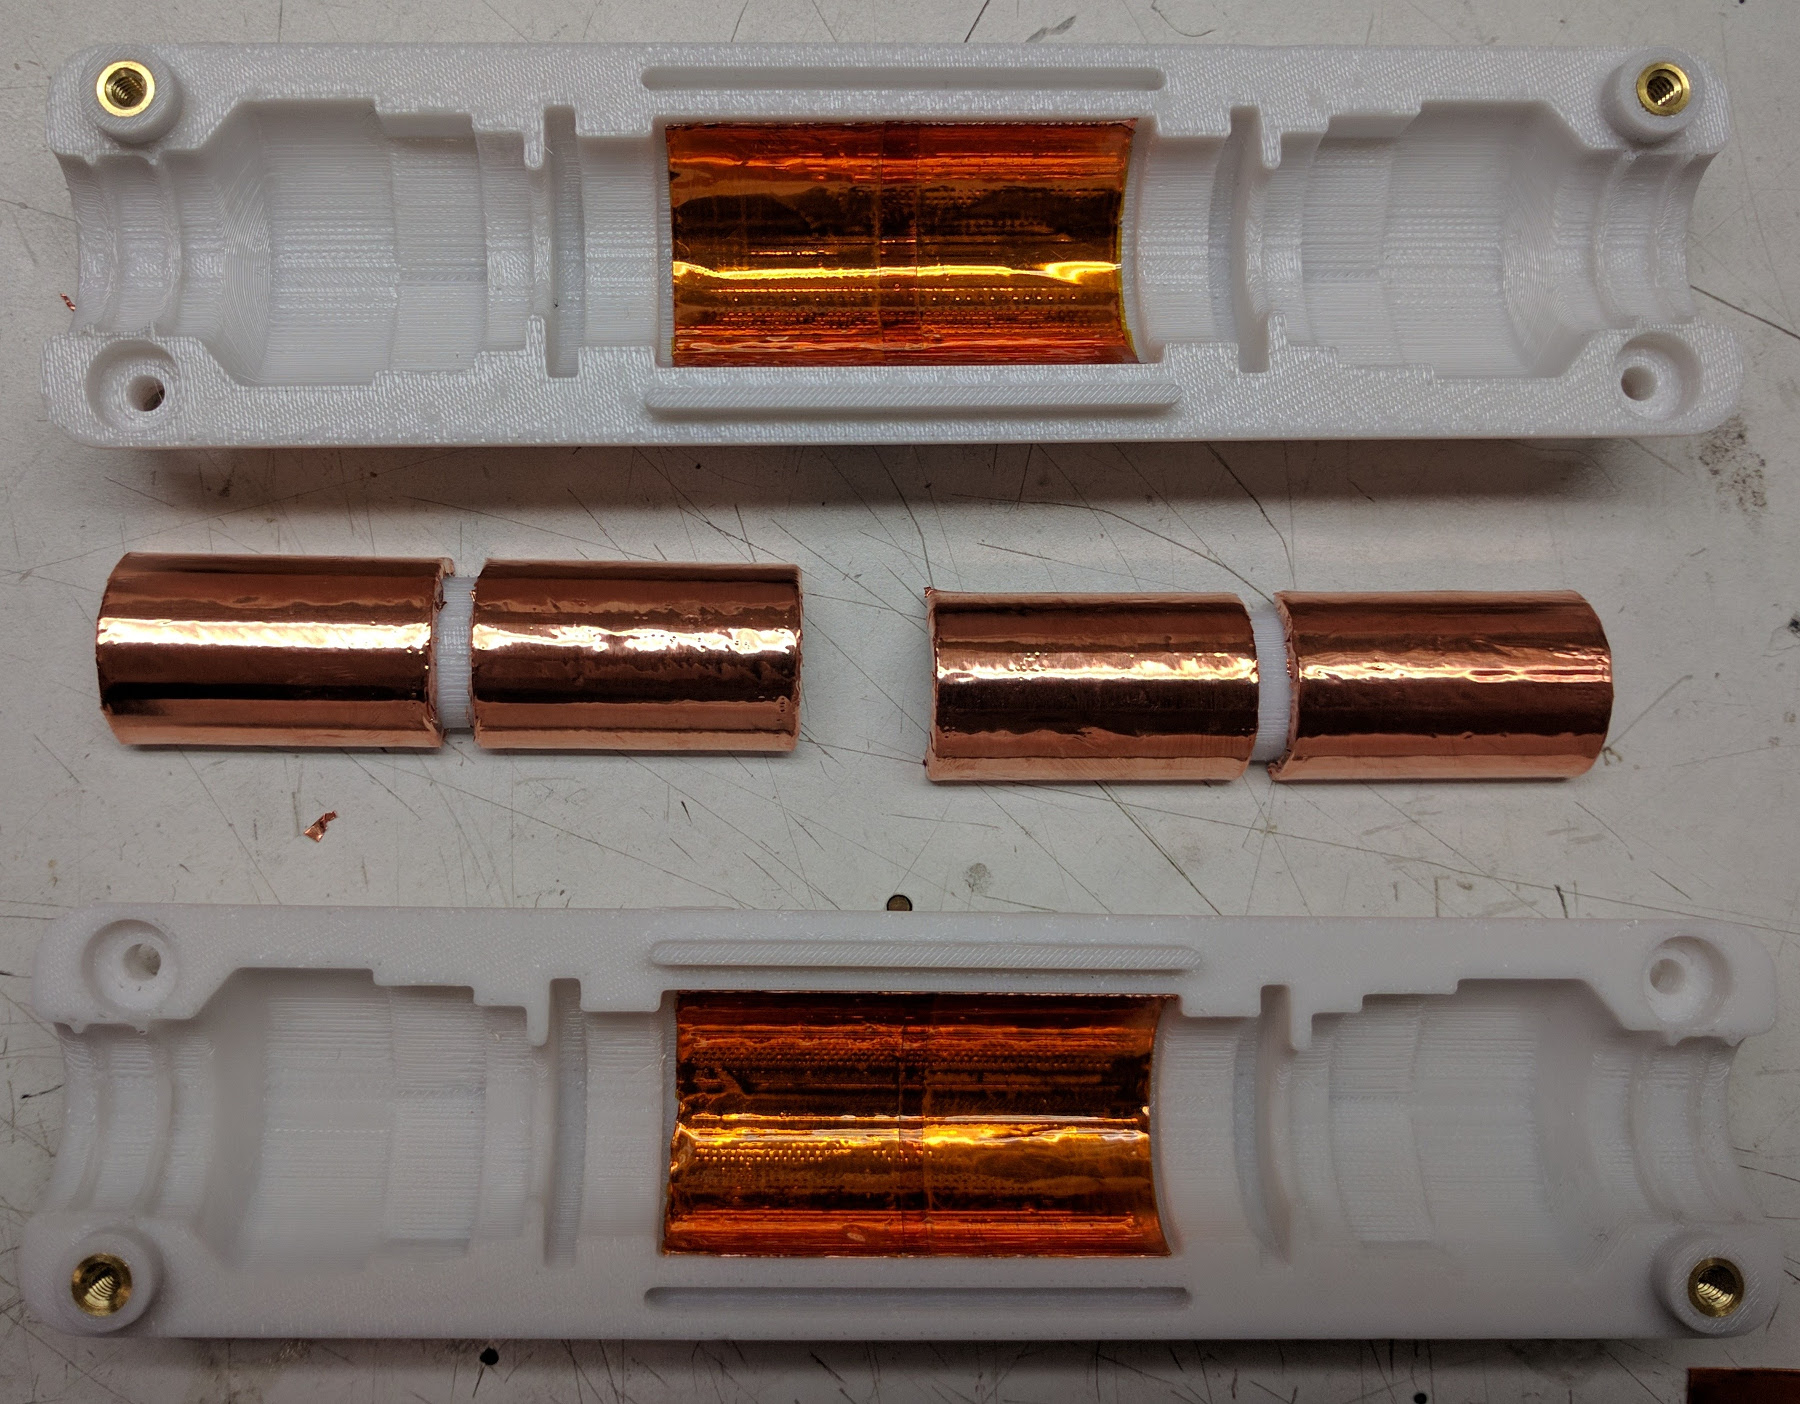
\includegraphics[width=6in]{figures/bazooka_parts.jpg}
\caption{Bazooka Balun before assembly.}
\label{fig:bazooka_parts}
\end{figure}

\begin{figure}
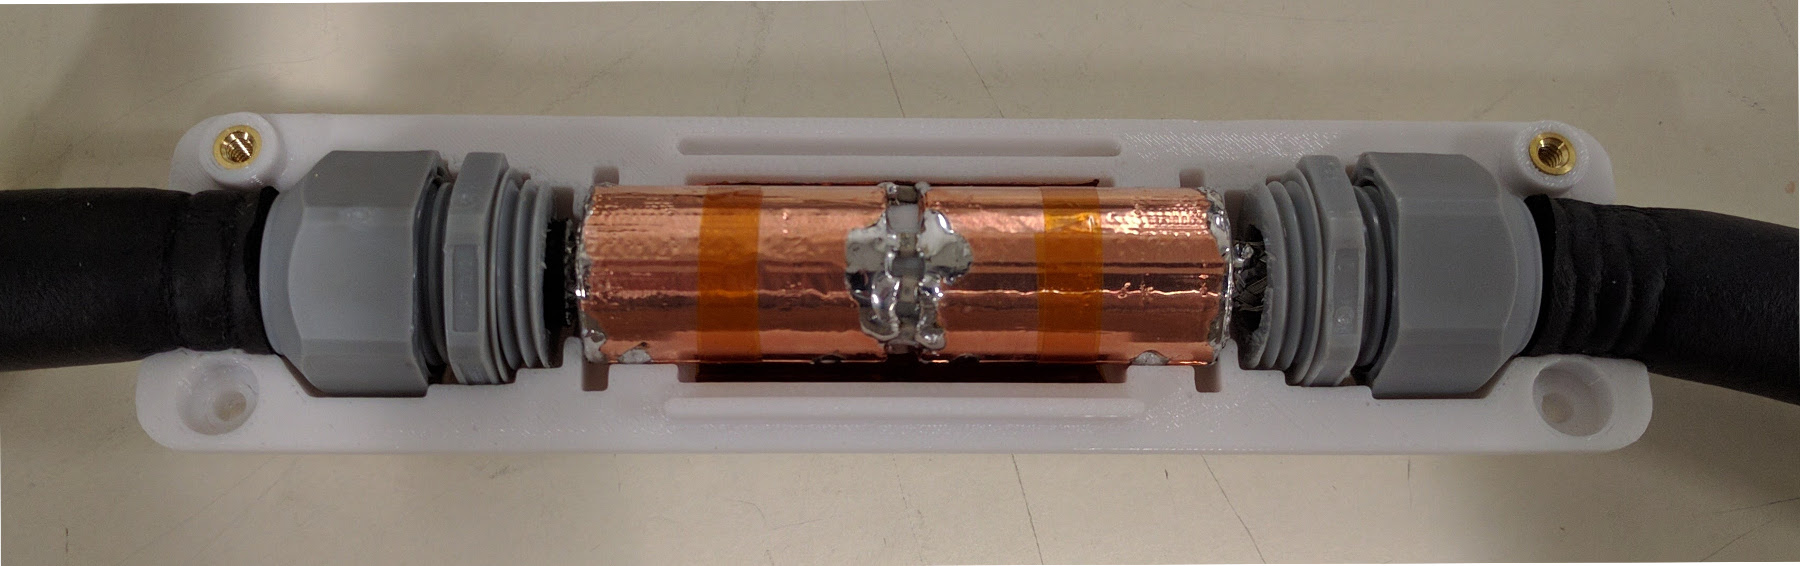
\includegraphics[width=6in]{figures/bazooka_assembled.jpg}
\caption{Completed bazooka balun with open enclosure.}
\label{fig:bazooka_assembled}
\end{figure}

\subsection{Trap Tuning}
Both of the cable trap types described are narrow band, and must be properly tuned to function. This is accomplished
through the use of a network analyzer and two current injection probes (fig. \ref{fig:bazooka_under_test}). Under the
right measurement conditions, a prominent dip (~$20dB$) in $|S_{12}|$ around the resonance frequency can be observed.

\begin{figure}
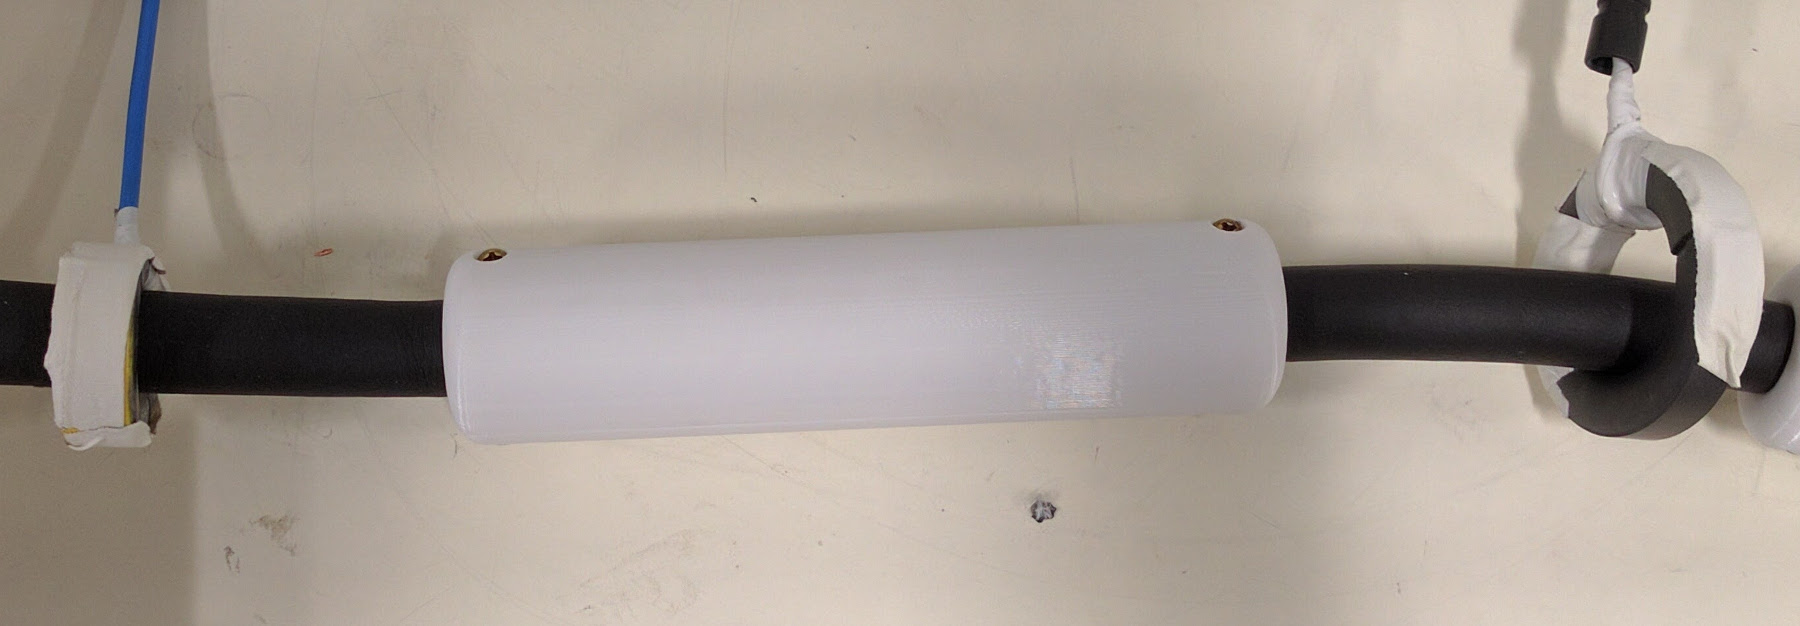
\includegraphics[width=6in]{figures/bazooka_under_test.jpg}
\caption{Cable trap with current injection probes.}
\label{fig:bazooka_under_test}
\end{figure}

\chapter{Loop Elements}

The same basic loop circuit, shown in figure \ref{fig:loop_schematic}, is duplicated 64 times to create the full array.
Here, I will discuss the purpose and function of each part of this circuit.

\section{Active Detuning}
The loop is a resonant circuit that is strongly coupled to the volume surrounding it. It is necessary to spoil this
resonance during the high power RF transmit pulses so that excessive currents are not induced in the loop. Such
unintended energy deposition could adversely affect transmit homogenaity, damage the array, or create a safety hazard.
This selective detuning is acheived by switching an inductor across one of the loop capacitors, creating a parallel
resonant tank that behaves as an open circuit in the loop at $\omega_L$.

A DC bias current of about $120mA$ is injected on the line marked BIAS in figure \ref{fig:loop_schematic}. This bias
current flows through a PIN diode, $D_1$, creating an RF short and effectively switching $L_{TRAP}$ across $C_{S3}$.
$L_{TRAP}$ is an adjustable air core inductor, and is hand tuned to resonate with $C_{S3}$ at precisely $\omega_L$. The 
parallel resonant circuit thus formed creates a virtual open ciruit in the loop, preventing current from flowing. As 
soon as the bias current is removed and the diode recovers, the trap is disabled and the loop once again becomes tuned.

\section{Passive Detuning}
The active detuning strategy is sufficient for assurance of image quality and protection from hardware damage, but a
passive method is required to ensure patient safety in the event of an electrical failure. The crossed diode pair $D_2$
clamps the voltage across $C_{S3}$ and $L_{TRAP}$ to safe levels, passively enabling the trap if the energy stored in
the loop gets too high. Other designs might also include RF fuses in the loop circuit, but the loops employed in this
array are all small enough that this was not necesarry.

\begin{figure}
    \centering
    \input{figures/loop_diagram.pdf_tex}
    \caption{Complete loop circuit schematic}
    \label{fig:loop_schematic}
\end{figure}

\section{Loop Model}
The essence of the wire loop receive elements used in this array is a damped series resonant circuit, shown in figure
\ref{fig:loop_model} A. The loop has a distributed inductance by nature of its geometry, and is broken at regular
intervals by discrete capacitors.  Wire and component resistances and (more importantly) inductive coupling to adjacent
conductive materials reduces the loop Q to a finite value. This effect is modelled by a series resistor with value
$R_{LOAD}=\sqrt{\frac{L}{C}}\cdot\frac{1}{Q}$

\section{Loop Circuit Output port}
Figure \ref{fig:loop_model} B shows the creation of an output port in the loop circuit. The total loop capacitance is
split into $C_P$, across which the output port is formed, and $C_S$. A series capacitor $C_M$ is added to one terminal
of the output port.

%For the purpose of further analisys, it is convenient to lump component impedances together into
%#three blocks: $Z_P$ (parallel imedance), $Z_S$ (series impedance), and $Z_M$ (matching impedance). These impedances are
%#defined in figure \ref{fig:loop_model} C.

\begin{figure}
    \centering
    \input{figures/loop_model.pdf_tex}
    \caption{Loop circuit models}
    \label{fig:loop_model}
\end{figure}

\section{Loop Circuit Analisys}
The loop ciruit has an input inpedance of $Z_{IN}$ at its port, as defined in equation \ref{eq:Z_IN}. This impedance can
be split into its real and imaginary parts, $R_{IN}$ and $X_{IN}$, shown in equations \ref{eq:R_IN} and \ref{eq:X_IN}.

\begin{equation} \label{eq:Z_IN}
    Z_{IN}=(jX_p)\parallel(jX_S+R_{L})+jX_M = \frac{1}{j\omega \cdot C_P + \frac{1}{R_{L}+j\omega\cdot L_{L} +
    \frac{1}{j\omega \cdot C_S}}} + \frac{1}{j\omega\cdot C_M}
\end{equation}

\begin{equation} \label{eq:R_IN}
    R_{IN}=\frac{{C_S}^2 R_{L}}{{C_P}^2 {C_S}^2 {L_{LOOP}}^2 \omega^4 + {C_P}^2 {C_S}^2 {R_{L}}^2
    \omega^2 - 2 {C_P}^2 C_S L_{L} \omega^2 + {C_P}^2 - 2 C_P {C_S}^2 L_{L} \omega^2 + 2 C_P C_S + {C_S}^2}
\end{equation}

\begin{equation} \label{eq:X_IN}
    X_{IN}= Im(Z_{IN}) = \frac{X_P ({R_L}^2 + X_S(X_P+X_S))}{{R_L}^2+(X_P+X_S)^2}+X_M
\end{equation}

\section{Loop Component selection}

\subsection{Loop Circuit Considerations}
\subsubsection{Minimizing Preamp Noise Figure}
The vendor supplied preamplifier is designed to achieve minimum noise figure when presented with a purely real
$50\Omega$ load at its input. Therefore, component values should be selected such that $R_{IN}=50\Omega$ and
$X_{IN}=0\Omega$. Call this optimal input impedance $Z_{IN_{OPT}}$.

\subsubsection{Preamp Decoupling}
Preamp decoupling is typicall achieved by resonating a capacitor in the loop ($C_P$ in figure \ref{fig:loop_model}) with
an inductor in series with one terminal of the output port (in the same position as $C_M$ in figure
\ref{fig:loop_model}) through the input of the preamplifier. In our case, however, the inductance is integrated into the
preamplifier itself. I measure the inductance of the preamplifer input to be roughly $130nH$ at $123.25 MHz$. The
details of the preamp topology are unavailible to me. I simply consider it to have an impedance of $Z_P$, which
is transformed to ${Z_P}'$ (as shown in equation \ref{eq:Z_PREAMP}) by the short length of coaxial cable (with
characteristic impeance $Z_0$) connecting the preamp to the loop.

\begin{equation} \label{eq:Z_PREAMP}
    {Z_P}'=Z_0 \cdot \frac{Z_P-j Z_0 \cdot \tan(2\pi\cdot\frac{L_{COAX}}{\lambda})}{Z_0 - j Z_P \cdot
    \tan(2\pi\cdot\frac{L_{COAX}}{\lambda})}
\end{equation}

\begin{equation} \label{eq:X_PREAMP}
    {X_P}'=Im({Z_P}')
\end{equation}
    
In any case, preamp decoupling is achieved when $C_P$, $C_M$, and the transformed preamp input impedance resonate
together, as defined in equation \ref{eq:preamp_decoupling_condition}.

\begin{equation} \label{eq:preamp_decoupling_condition}
    X_P + X_M +{X_P}' = 0
\end{equation}


\subsection{Loop Resonance}

I define loop resonance as occuring at a frequency $\omega_0$ where $X_P + X_S = 0$. In this case, the equations for
$R_{IN}$ and $X_{IN}$ simplify to equations \ref{eq:R_IN_RES} and \ref{eq:X_IN_RES} respectively. Rearranging equation
\ref{eq:R_IN_RES} into equation \ref{eq:X_P_RIN} gives a formula for setting the value of $R_IN$ on resonance; however,
it is then impossible to select $X_M$ to simultaneously achieve zero $X_{IN}$ and satisfy the preamp decoupling conditon
(equation \ref{eq:preamp_decoupling_condition})


\begin{equation} \label{eq:R_IN_RES}
    R_{IN}\big|_{\omega=\omega_0}=\frac{{X_P}^2}{R_L} = \frac{{X_S}^2}{R_L} 
\end{equation}

\begin{equation} \label{eq:X_IN_RES}
    X_{IN}\big|_{\omega=\omega_0}=X_P+X_M=-X_S+X_M
\end{equation}

\begin{equation} \label{eq:X_P_RIN}
    X_{P}(R_{IN})\big|_{\omega=\omega_0}=-\sqrt{R_{LOAD} \cdot R_{IN}} 
\end{equation}

\subsection{Off resonance behavior}
It is not necessary that the loop be tuned to resonate precisely at the frequency of interest. The position of
$\omega_0$ relative to that of the Lamor frequency $\omega_L$ is another variable that we can manipulate to achieve the
desired loop circuit characteristics.

\subsubsection{Choosing $X_P$}
Consider choosing $X_P=-\sqrt{\alpha\ \cdot Z_{OPT} \cdot R_{LOAD}}$, so that the value of $R_{IN}$ on resonance is a
factor of $\alpha$ larger than $Z_{OPT}$. Substituting this value into eq. \ref{eq:R_IN}, we get a new equation for
$R_{IN}$: eq. \ref{eq:R_IN_alpha}. The frequency dependent value of $R_{IN}$ is plotted in figure
\ref{fig:impedance_plot}

\begin{equation} \label{eq:R_IN_alpha}
    R_{IN}\big|_{X_P=-\sqrt{\alpha Z_{OPT} R_{LOAD}}} = \frac{\alpha Z_{OPT} {R_{LOAD}}^2}{{R_L}^2 + \alpha Z_{OPT} R_{LOAD} - 2\sqrt{\alpha Z_{OPT} R_{LOAD}} X_S + {X_S}^2}
\end{equation}

\subsubsection{Choosing $X_S$}
Indeed, when $X_P=-\sqrt{\alpha Z_{OPT} R_{LOAD}}$ and $X_S=\sqrt{\alpha Z_{OPT} R_{LOAD}}$, eq.  \ref{eq:R_IN_alpha}
reduces to $R_{IN} = \alpha \cdot Z_{OPT}$.  But on either side of this resonant peak, there is a single frequency at
which $R_{IN} = Z_{OPT}$. Solving \ref{eq:R_IN_alpha} for the two values of $X_S$ at which this occurs, we get: $$X_S =
\sqrt{\alpha Z_{OPT} R_{LOAD}} \pm R_{LOAD} \sqrt{\alpha - 1}$$ We choose the minus sign in this expression, and thus
achieve $R_{IN} = Z_{OPT}$ at a frequency below $\omega_0$, because this makes the sytem of equations in the next step
solvable.

\subsubsection{Choosing $\alpha$ and $X_M$}
The only remaining free parameters are $\alpha$ and $X_M$.  They must be chosen to achieve purely real input inpedance
($X_{IN} = 0$) and preamp decoupling ($X_P + X_M +{X_P}' = 0$). Plugging in the values of $X_P$ and $X_S$ that we've
selected so far into these two requirements, we get a system of equations with a singe set of solutions:
$$
\begin{aligned}
    Z_{OPT} \sqrt{\alpha - 1} - \sqrt{\alpha Z_{OPT} R_{LOAD}} + X_M &= 0\\
    -\sqrt{\alpha Z_{OPT}} + X_M + {X_P}' &= 0
\end{aligned}
\implies
\begin{aligned}
    \alpha &= 1 + \frac{{X_P}'^2}{Z_{OPT}}\\
    X_M &= \sqrt{\frac{R_{LOAD}}{Z_{OPT}} ({X_P}'^2 + {Z_{OPT}}^2} - {X_P}'
\end{aligned}
$$

\subsection{Optimal Component values}



\begin{figure}
    \centering
    \input{figures/impedance_plot.pdf_tex}
    \caption{Loop impedances vs. frequency with optimal component values}
    \label{fig:impedance_plot}
\end{figure}

\chapter{Testing}
The aim of this project was to create a custom coil that performs better than existing arrays in a
particular application. Our primary means of evaluating relative performance is direct comparison of two related
performance metrics: SNR maps and SENSE geometry factor (g-factor) maps. A brief discussion of each follows. For a
complete treatment, see the original SENSE paper: \cite{Pruessmann1999}.

\section{Signal to Noise Ratio Maps}
The MR signal to noise ratio provided by any coil or coil array varies as a function
of space. A a heatmap of SNR in a given plane is a useful visual tool that can be used to judge wheter a coil is well
suited to imaging in a particular region of interest such as the fetal brain or placenta. A SNR map is easy to generate
for a single coil. One can simply run an imaging sequence with intrincicly high SNR twice; once with an initial RF
excitation and once without. The first sequence should produce an image that is dominated by the MR signal, and the
second sequence produces a noise only image. A SNR map in conventionally defined SNR units is obtained by dividing the
first image by the standard deviation of the noise only image.

Generating SNR maps for multi coil arrays is less straigtforward, and depends on the method used to combine data from
indidiual elements. The Roemer paper \cite{Roemer90} describes an optimal way of combining array coil data in the
spatial domain that results in maximum SNR and normalized noise intensity in every voxel of the resulting image.  First,
a complete image is acquired and reconstructed from every element in the array. Next, a sample of pure noise data is
acquired to generate a channel noise correlation matirx $\Psi$, of which a single element $Psi_{ij}$ is the noise
correlation coefficient between receivers $i$ and $j$. Next, the individual coil images are combined on a voxel by voxel
basis. For a single voxel, arrange the values $S_i$ of that voxel in each of the indivudual coil images in a vector $S$.
Similarly, arrange the sensitivities of each coil to the voxel under consideration in a vector $C$.The matrix equation
for the voxel intensity in the optimal SNR uniform noise image is then \ref{eq:I_OPT}. If the individual coil images
have sufficiently high SNR, then $S$ serves as a good approximation of $C$, and equation simplifies to \ref{eq:I_COV}.
If it is assumed that there is no noise correlation between distinct channels, $\Psi$ becomes the identity matrix, and
the optimal SNR formula simplifies to \ref{eq:I_RSOS}. This is equivilent to summing the squared magnitudes of the
uncombined images, then taking the square root of the result.

\begin{equation} \label{eq:I_OPT}
I_{OPT}=\frac{C^H\Psi^{-1}S}{\sqrt{C^H\Psi^{-1}C}}
\end{equation}

\begin{equation} \label{eq:I_COV}
I_{COV}=\sqrt{S^H\Psi^{-1}S}
\end{equation}

\begin{equation} \label{eq:I_RSOS}
I_{RSOS}=\sqrt{S^{H} S}
\end{equation}

TODO:SNR equations

\section{SENSE Geometry Factor}

\chapter{Methods}

\section{Bench Tests}
\subsection{Intercoil Coupling and Reflection Coefficient Measurements}
A network analyzer connected directly to loop output ports was used to measure coupling between neighboring coil
elements ($S_{12}$), and to measure individual coil output reflection coefficients ($S{11}$). For each of theses tests,
the output power of the network analyzer was reduced to -25dBm and the coil was appropriately loaded by a test phantom.
This test configuration was used during the iterative geometric decoupling adjustment process, where the loops are
manually bent and reconfigured to minimize neighbor-to-neighbor coupling.

\subsection{Loop Detuning and Preamp Decoupling Verification}
The active detune capability and preamp decoupling performance were  tuned and characterized using a pair of decoupled
($S_{12}<70dB$) inductive probes loosely coupled to the loop under test. In this arrangement, the $S_{12}$ measurement
between the two probes is directly proportional to the current flowing in the loop \cite{Reykowski1995}. Both the active
detune capability and preamplifier decoupling strategy work by introducing a second resonance near the loop resonance
frequency, which "splits" the loop resonance into two peaks above and below the initial resonance frequency. The null
between these peaks is moved to $\omega_L$ by adjustment of a tunable component. For the active detune strategy, this
tunable component is an adjustable air-core inductor ($L_{TRAP}$ in fig. \ref{fig:loop_schematic}). For preamp
decoupling, it is a trim capacitor ($C_M$ in fig.  \ref{fig:loop_schematic}).

\section{MRI Data Acquisition and Reconstruction}
Images of the pregnant abdominal phantom were acquired for using both the 64 channel fetal coil and the standard
combination of 16 channels from a 32 channel spine array and all channels from an 18 channel flexible body array. Three
orthogonal slices (transverse, coronal, and sagital) intersecting the fetal brain compartment were carefully duplicated
using both array configurations. An extremely high SNR PD weighted 2DGRE sequence ($TR=3500ms, TE=4ms, FA=45^{\circ},
FOV=400mm, \delta \approx 2mm \times 2mm \times 7mm, BW=180Hz/px$) was chosen so that each of the uncombined coil images
has decent SNR ($>20$) in the deep central region of the fetal brain compartment, and thus can be taken as an accurate
approximation of a coil sensitivity map \cite{Roemer90}. The same sequence was run with the reference TX voltage set to
$0V$ to acquire noise-only data for the generation of a noise covariance matrix $\Psi$. Data were acquired on a 3T
Magnetom Skyra System (Siemens Healthcare, Erlangen, Germany).

Covariance weighted SNR maps and SENSE g-factor maps were computed offline using the resulting raw data. For the fetal
coil, single channel SNR maps were generated by dividing each of the 64 uncombined coil images by the standard deviation
of a corresponding noise only image. The mean value of each single channel SNR map was computed inside an ROI ($A=29$
voxels) in the fetal brain region of the anthropomorphic phantom as a means of assessing the relative importance of each
component in the array geometry.



\chapter{Results}
\section{SNR Maps}

\begin{figure}
\makebox[\textwidth][c]{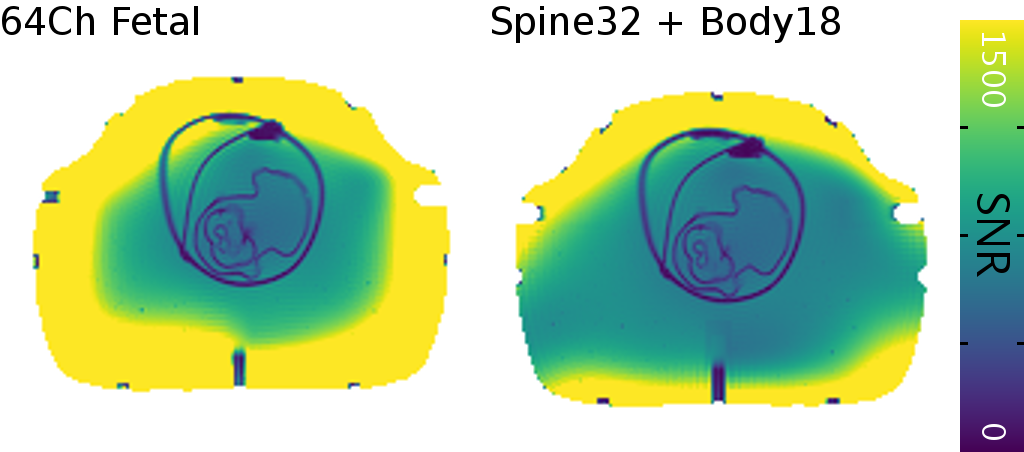
\includegraphics{figures/SNR_TRA_0-1500_viridis.png}}
\caption{Comparative Covariance Weighted SNR Maps, Transverse Slice Through Fetal Phantom Brain.}
\label{fig:SNR_tra}
\end{figure}

\begin{figure}
\makebox[\textwidth][c]{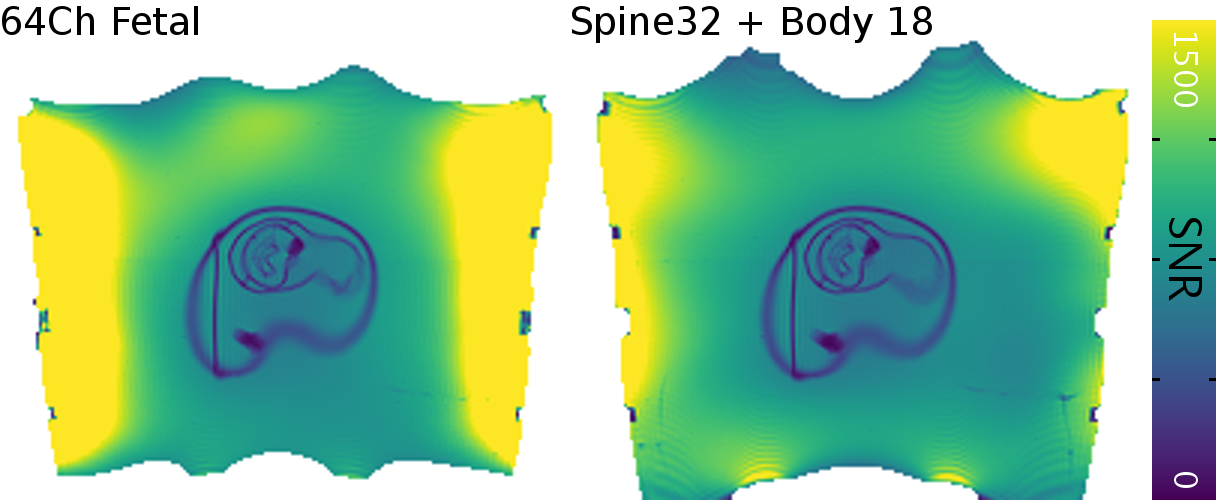
\includegraphics{figures/SNR_COR_0-1500_viridis.png}}
\caption{Comparative Covariance Weighted SNR Maps, Coronal Slice Through Fetal Phantom Brain.}
\label{fig:SNR_cor}
\end{figure}

\begin{figure}
\makebox[\textwidth][c]{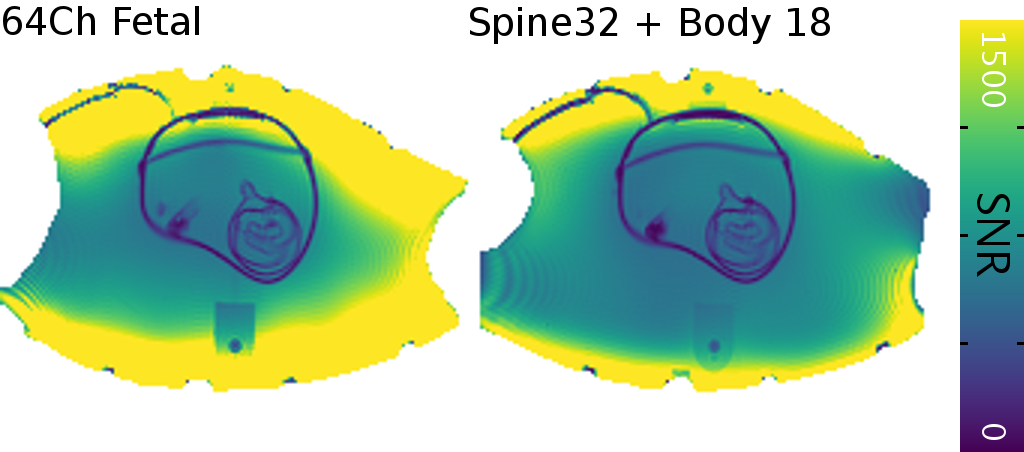
\includegraphics{figures/SNR_SAG_0-1500_viridis.png}}
\caption{Comparative Covariance Weighted SNR Maps, Sagital Slice Through Fetal Phantom Brain.}
\label{fig:SNR_sag}
\end{figure}



\section{G-Factor Maps}

\begin{figure}
\makebox[\textwidth][c]{\includegraphics{figures/{gfactor_TRA_RL_2-3-4-5-6_0.5-1_viridis}.png}}
\caption{Comparative Inverse SENSE G-Factor Maps, Transverse Slice Through Fetal Phantom Brain, Acceleration in Right-Left Direction.}
\label{fig:gfactor_tra_rl}
\end{figure}

\begin{figure}
\makebox[\textwidth][c]{\includegraphics{figures/{gfactor_TRA_AP_2-3-4-5-6_0.5-1_viridis}.png}}
\caption{Comparative Inverse SENSE G-Factor Maps, Transverse Slice Through Fetal Phantom Brain, Acceleration in Anterior-Posterior Direction.}
\label{fig:gfactor_tra_ap}
\end{figure}

\begin{figure}
\makebox[\textwidth][c]{\includegraphics{figures/{gfactor_COR_RL_2-3-4-5-6_0.5-1_viridis}.png}}
\caption{Comparative Inverse SENSE G-Factor Maps, Coronal Slice Through Fetal Phantom Brain, Acceleration in Right-Left Direction.}
\label{fig:gfactor_cor_rl}
\end{figure}

\begin{figure}
\makebox[\textwidth][c]{\includegraphics{figures/{gfactor_COR_HF_2-3-4-5-6_0.5-1_viridis}.png}}
\caption{Comparative Inverse SENSE G-Factor Maps, Coronal Slice Through Fetal Phantom Brain, Acceleration in Head-Foot Direction.}
\label{fig:gfactor_cor_hf}
\end{figure}

\begin{figure}
\makebox[\textwidth][c]{\includegraphics{figures/{gfactor_SAG_HF_2-3-4-5-6_0.5-1_viridis}.png}}
\caption{Comparative Inverse SENSE G-Factor Maps, Sagital Slice Through Fetal Phantom Brain, Acceleration in Head-Foot Direction.}
\label{fig:gfactor_sag_hf}
\end{figure}

\begin{figure}
\makebox[\textwidth][c]{\includegraphics{figures/{gfactor_SAG_AP_2-3-4-5-6_0.5-1_viridis}.png}}
\caption{Comparative Inverse SENSE G-Factor Maps, Sagital Slice Through Fetal Phantom Brain, Acceleration in Anterior-Posterior Direction.}
\label{fig:gfactor_sag_ap}
\end{figure}

\section{Per-Element SNR}
\begin{figure}
\makebox[\textwidth][c]{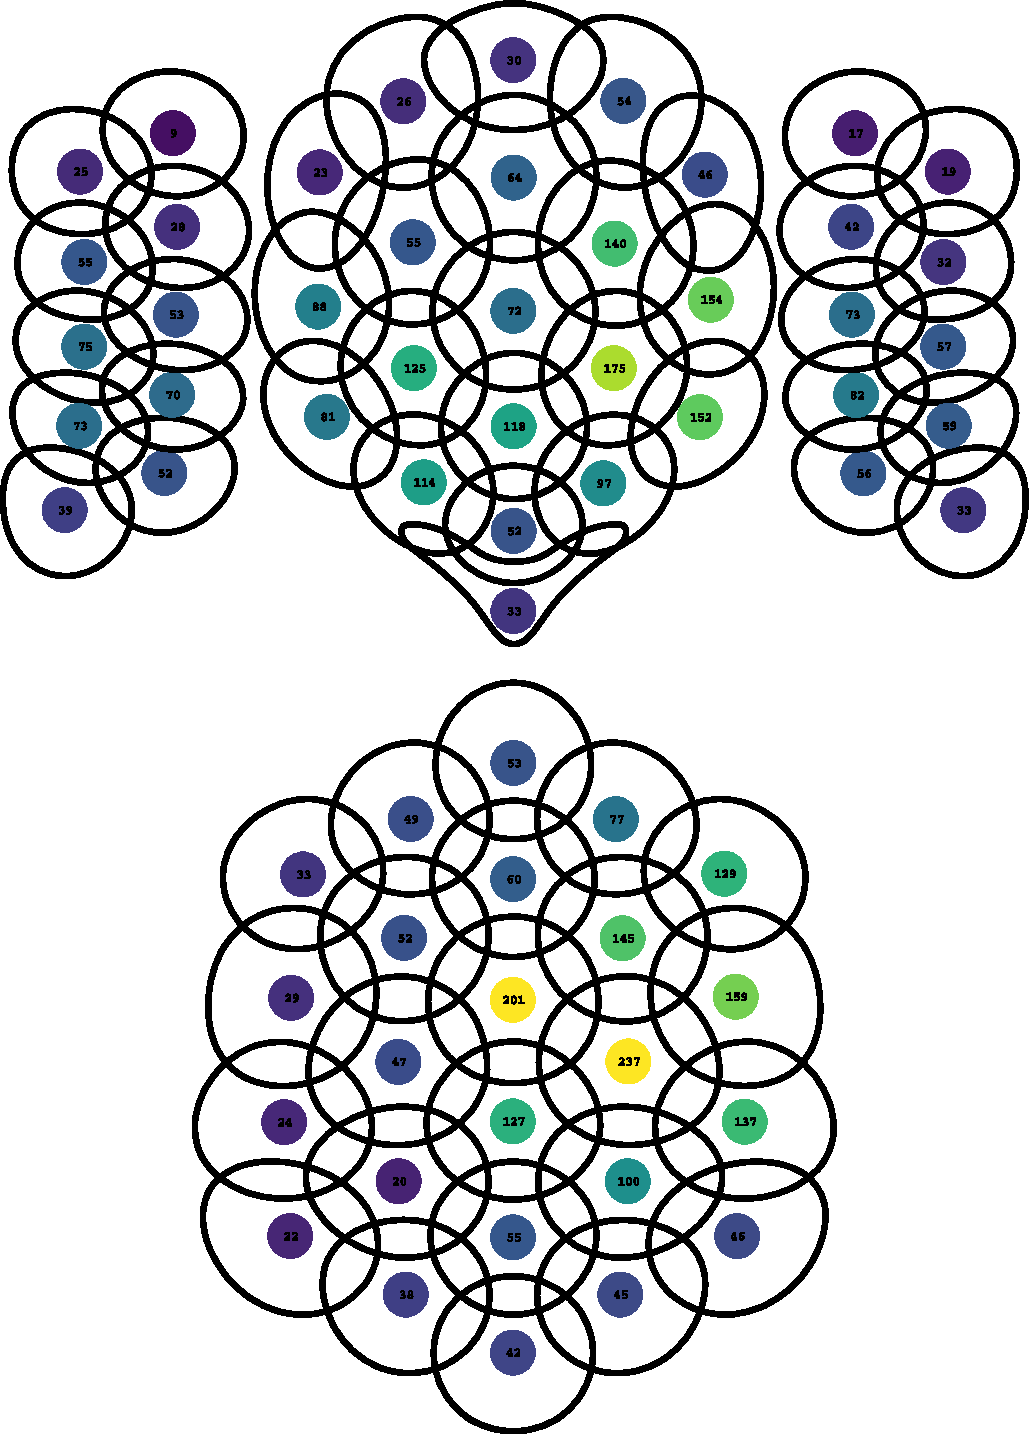
\includegraphics{figures/loop_snr_contributions.pdf}}
\caption{Single Element SNR values Inside the Fetal Phantom Brain}
\label{fig:loop_snr_contributions}
\end{figure}

\chapter{Discussion}
The modest SNR improvement seen in unaccelerated imaging is likely attributed to the deep (nearly central) location of
the fetal head where coil arrays with more than 16 elements already approach the ultimate SNR available
\cite{Wiesinger2004}.  Nonetheless, because the SNR is achieved with array elements with higher spatial frequency
sensitivity profiles, there is an improvement in acceleration capability. 

%% This defines the bibliography file (main.bib) and the bibliography style.
%% If you want to create a bibliography file by hand, change the contents of
%% this file to a `thebibliography' environment.  For more information 
%% see section 4.3 of the LaTeX manual.
\begin{singlespace}
\bibliography{main}
\bibliographystyle{plain}
\end{singlespace}

\end{document}

